%% right-side equation numbering, 12 point font, print one-sided 
%\documentclass[reqno,12pt,oneside]{report} 
\documentclass[12pt,letterpaper,oneside]{book}

% Use my personal style sheet
%\usepackage{tomf}         

\usepackage{color}
\usepackage{times}
\usepackage{amsmath,amsfonts,amssymb}
\usepackage{amsthm}   % for theorems

%\usepackage{graphics}
\usepackage{graphicx} % This is preferred. %> convert image.png image.eps

% To allow argmin, argmax to write subscript below, not to the right and down.
\newcommand{\argmin}{\operatornamewithlimits{argmin}}
\newcommand{\argmax}{\operatornamewithlimits{argmax}}

%%%%%%%%%%%%%%%%%%%%%%%%%%%%%%%%%%%%%%%%%%%%%%%%%%%%%%%%%%%%%%%%%%%%%%%%%%%%%%%
\usepackage{listings}

\definecolor{dkgreen}{rgb}{0,0.6,0}
\definecolor{gray}{rgb}{0.5,0.5,0.5}
\definecolor{mauve}{rgb}{0.58,0,0.82}

\lstset{ 
  backgroundcolor=\color{white},  % choose the background color; \usepackage{[x]color} 
  basicstyle=\footnotesize\ttfamily,       % the size of the fonts that are used for the code
  breakatwhitespace=false,        % sets if automatic breaks should only happen at whitespace
  breaklines=true,                % sets automatic line breaking
  captionpos=b,                   % sets the caption-position to bottom
  commentstyle=\color{dkgreen},   % comment style
  deletekeywords={...},           % if you want to delete keywords from the given language
  escapeinside={\%*}{*)},         % if you want to add LaTeX within your code
  %extendedchar=true,              % lets you use non-ASCII characters; for 8-bits encodings
  frame=single,                   % adds a frame around the code
  keywordstyle=\color{blue},      % keyword style
  language=Python,                % the language of the code
  morekeywords={*,...},           % if you want to add more keywords to the set
  numbers=none,                   % location of line-numbers; (none, left, right)
  numbersep=5pt,                  % how far the line-numbers are from the code
  numberstyle=\tiny\color{gray},  % the style that is used for the line-numbers
  rulecolor=\color{black},        % if not set, the frame-color may be changed on line-breaks  
  showstringspaces=false,         % underline spaces within strings only
  showtabs=false,                 % show tabs within strings adding particular underscores
  stepnumber=2,                   % the step between two line-numbers. If 1, each line numbered
  stringstyle=\color{mauve},      % string literal style
  tabsize=2,                      % sets default tabsize to 2 spaces
  title=\lstname                  % show the filename of files included with \lstinputlisting; 
}

%%%%%%%%%%%%%%%%%%%%%%%%%%%%%%%%%%%%%%%%%%%%%%%%%%%%%%%%%%%%%%%%%%%%%%%%%%%%%%%

% Various theorem environments. All of the following have the same numbering
% system as theorem.

\theoremstyle{plain}
\newtheorem{theorem}{Theorem}
\newtheorem{prop}[theorem]{Proposition}
\newtheorem{corollary}[theorem]{Corollary}
\newtheorem{lemma}[theorem]{Lemma}
\newtheorem{question}[theorem]{Question}
\newtheorem{conjecture}[theorem]{Conjecture}
\newtheorem{assumption}[theorem]{Assumption}

\theoremstyle{definition}
\newtheorem{definition}[theorem]{Definition}
\newtheorem{notation}[theorem]{Notation}
\newtheorem{condition}[theorem]{Condition}
\newtheorem{example}[theorem]{Example}
\newtheorem{introduction}[theorem]{Introduction}

\theoremstyle{remark}
\newtheorem{remark}[theorem]{Remark}

% Numbers theorems "x.y" where x is the section number, y is the theorem number
\numberwithin{theorem}{chapter}     

%%%%%%%%%%%%%%%%%%%%%%%%%%%%%%%%%%%%%%%%%%%%%%%%%%%%%%%%%%%%%%%%%%%%%%%%%%%%%%

%% This command creates a box marked ``To Do'' around text.
%% To use type \todo{  insert text here  }.

\newcommand{\todo}[1]{\vspace{5 mm}\par \noindent
\marginpar{\textsc{To Do}}
\framebox{\begin{minipage}[c]{0.95 \textwidth}
\tt\begin{center} #1 \end{center}\end{minipage}}\vspace{5 mm}\par}

\def\startabstractpage#1{% This formats the optional in-dissertation abstract - jg
 \newpage
 \setcounter{page}{1}   % -- begin with "i" TRF
 \addcontentsline{toc}{chapter}{ABSTRACT}
 \@restonecolfalse\if@twocolumn\@restonecoltrue\onecolumn\fi
 \hbox{ }
 \twoinmar
 \centerline{ABSTRACT}
 \vspace{0.4in}
 \noindent #1
 \vspace{0.25in}\\
}

%% Allow " quotes to be used directly.
%%%%%%%%%%%%%%%%%%%%%%%%%%%%%%%%%%%%%%%%%%%%%%%%%%%%%%%%%%%%%%%%%%%%%%%%%%%%%%%%%%%%%%%%%%

\begin {document}

%%%%%%%%%%%%%%%%%%%%%%%%%%%%%%%%%%%%%%%%%%%%%%%%%%%%%%%%%%%%%%%%%%%%%%%%%%%%%%%%%%%%%%%%%%

% Page numbering. If you don't include a frontispiece or copyright
% page, you'll need to change this for two-sided printing.
\makeatletter
\if@twoside \setcounter{page}{4} \else \setcounter{page}{1} \fi
\makeatother

% Abstract
%\startabstractpage{\input{abstract}}

% Table of contents, list of figures, etc.
\tableofcontents     % Required
\listoftables        % Required if there is more than one table
\listoffigures       % Required if there is more than one figure
%\listofmaps          % Required if there is more than one map
%\listofappendices    % Required if there is more than one appendix
%\listofabbreviations % Optional. Abbreviations should be stored in a file named abbr.tex

% Optional in-dissertation Abstract Page
%\startabstractpage{The Title of Your Dissertation}{Your Name}{Chair: Albert Einstein}
%\input{Abstract/Abstract}
%\label{Abstract}

%%%%%%%%%%%%%%%%%%%%%%%%%%%%%%%%%%%%%%%%%%%%%%%%%%%%%%%%%%%%%%%%%%%%%%%%%%%%%%%%%%%%%%%%%%
%\startthechapters 
% The individual files for each of the chapters are put here.
% Save each chapter of your thesis to a seperate tex file
% and then use the \input command to include this file in your
% thesis.  For instance you can save a file to "intro.tex" and 
% then type \input{intro}. 
%%%%%%%%%%%%%%%%%%%%%%%%%%%%%%%%%%%%%%%%%%%%%%%%%%%%%%%%%%%%%%%%%%%%%%%%%%%%%%%%%%%%%%%%%%
% use \input   for non-page-break % and \include for page-break

\chapter{Introduction}
figure \ref{fig:gaussian}. Here, no presumption is yet made about the kind of distribution for the source (random) variable $X$. 

\begin{figure}
  \centering
  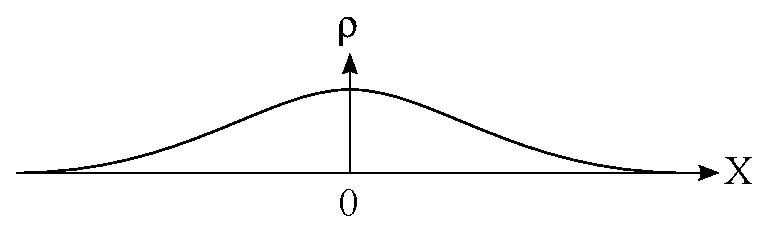
\includegraphics{Images/gaussian.eps}
  \caption[Distribution of source variable $X$]
          {Distribution of source variable $X$}
  \label{fig:gaussian}
\end{figure}

Following Dineen \cite{dineen00}

\chapter{Numeric Computation}
\section{Numeric Representation}

\begin{figure}
  \centering
  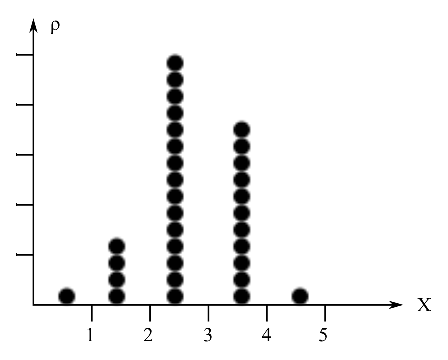
\includegraphics{Images/SkewedNormalHistogram.eps}
  \caption[Example Sample]
          {Example Sample}
  \label{fig:SkewedNormalHistogram2}
\end{figure}

\begin{figure}
  \centering
  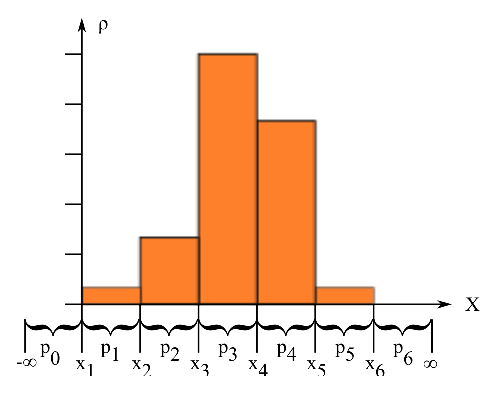
\includegraphics{Images/ArbitraryHistogram.eps}
  \caption[1D Numeric Random Variable]
          {1D Numeric Random Variable}
  \label{fig:ArbitraryHistogram}
\end{figure}

Given a sample of a random variable and a partition of the support space as in figure \ref{fig:SkewedNormalHistogram2} a histogram forms a natural summary. In RICO, a method of representing a one dimensional continuous random variable numerically is suggested in figure \ref{fig:ArbitraryHistogram}. Since random variables may be both discrete and continuously distributed at the same time a pair of parallel arrays is used programmatically,
\begin{align*}
X \sim \begin{cases}
    X_c = \begin{cases}
    (x_0 = -\infty, x_1, x_2, ..., x_n, x_{n+1} = \infty)\\
    (p_0, p_1, ..., p_n, 0)
    \end{cases}\\
    X_d = \begin{cases}
    (y_1, y_2, ..., x_m)\\
    (q_1, q_2, ..., q_m)
    \end{cases}
  \end{cases}
\end{align*}
where
\begin{align*}
-\infty < x_1 < ... < x_n < \infty
\end{align*}
The endpoints for the continuously distributed portion of $X$, $X_c$, are assumed to be $\pm \infty$ with $n$ partition endpoints between. The $p_i$ values are defined as
\begin{align*}
p_i := \begin{cases}
  P(x_i < X_c < x_{i+1}) & \text{ if } i \in \{1, ..., n-1\}\\
  P(X_c < x_1) & \text{ if } i = 0\\
  P(x_n < X_c) & \text{ if } i = n+1
  \end{cases}
\end{align*}
and the $q_j$ values are defined as
\begin{align*}
q_j := P(X_d = y_j) \text{ for } j \in \{1, ..., m\}
\end{align*}

For an example of RICO in action, let $X \sim N(0,1)$ numerically represented. New random variables such as $e^X$ and $X^{1.25}$ can be created and graphed, see table \ref{fig:OneDimFunction}. The code used to generate the graphs is

\begin{lstlisting}
X = NormalNumeric(0,1,1000)
Plot(exp(X))
Plot(X**1.25)
\end{lstlisting}


\begin{table}
\begin{center}
\begin{tabular}{cc}
$X$ & $e^X$\\
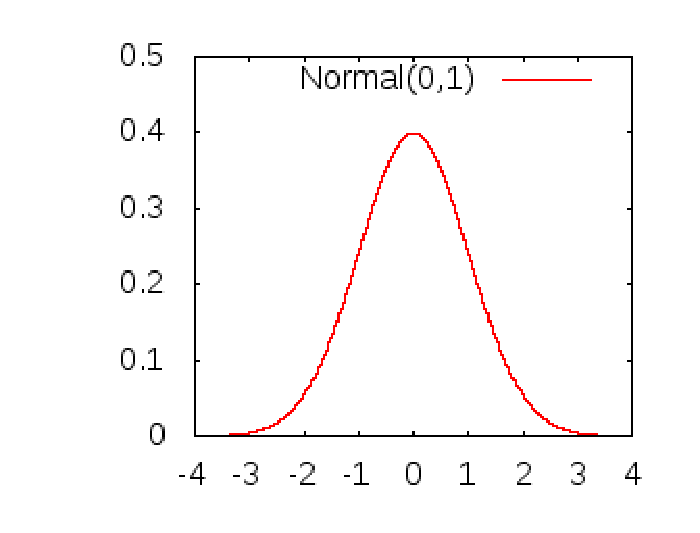
\includegraphics[width=2in]{Images/NormalDSN.eps} &
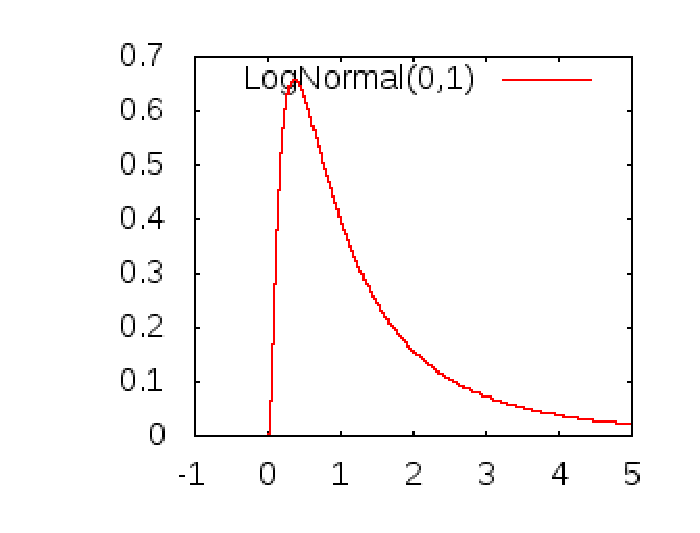
\includegraphics[width=2in]{Images/LogNormalDSN.eps} \\
$X$ & $X^{1.25}$\\
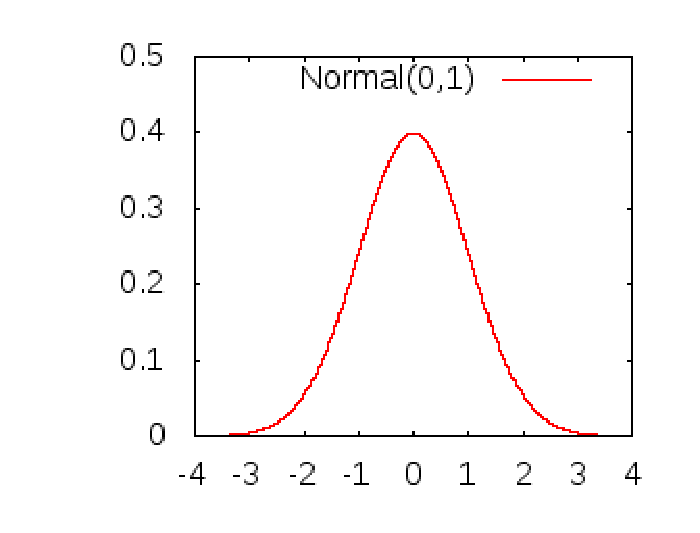
\includegraphics[width=2in]{Images/NormalDSN.eps} &
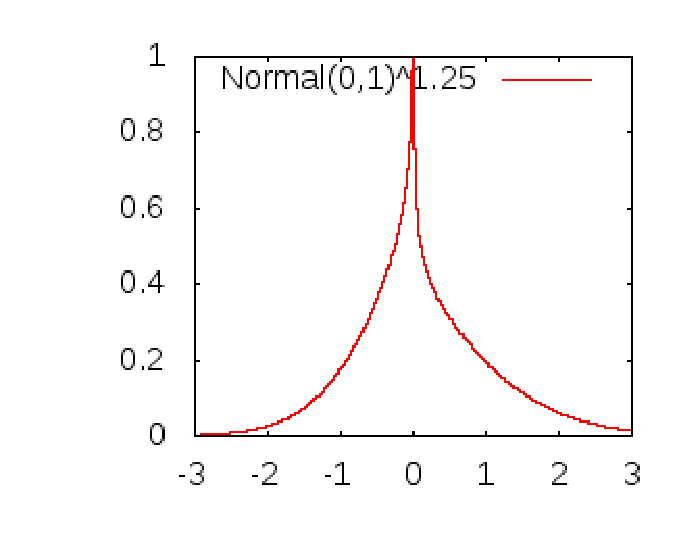
\includegraphics[width=2in]{Images/PowerNormalDSN.eps} \\
\end{tabular}
\end{center}
\caption[Standard Normal $X$, $e^X$, $X^{1.25}$]
        {Standard Normal $X$, $e^X$, $X^{1.25}$}
\label{fig:OneDimFunction}
\end{table}

\begin{figure}
  \centering
  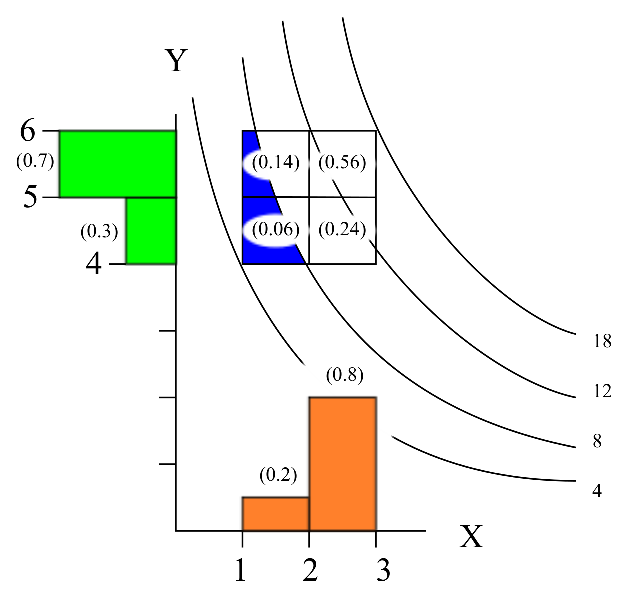
\includegraphics[width=3in]{Images/AxB_partitioned.eps}
  \caption[Piecewise Continuous X times Y]
          {Piecewise Continuous X times Y}
  \label{fig:AxB_Partitioned}
\end{figure}

Illustrative example of multiplication of two piecewise continuous random variables $X$ and $Y$.  Referring to figure \ref{fig:AxB_Partitioned}, the following conditions hold for $X$ and $Y$,
\begin{align*}
P(1 < X < 2) = 0.2 && P(2 < X < 3) = 0.8\\
P(4 < Y < 5) = 0.3 && P(5 < Y < 6) = 0.7
\end{align*}
and the probability densities are super-imposed on the joint density distribution of $(X,Y)$. For illustrative purposes a partition of the $XY$ random variables is chosen as $(4,8,12,18)$ to coincide with the corners of the non-zero probability density region of $(X,Y)$. Each partition endpoint $\{4,8,12,18\}$ corresponds to an iso-probability level curve identified in the figure \ref{fig:AxB_Partitioned}. Notice that in the case of multiplication the level curves are hyperbolas. To compute the numeric random variable $XY$ given the partition $(4,8,12,18)$, calculate the area between level curves within joint probability rectangles. In particular, to compute $P(4 < XY < 8)$ one must find the fractional area of each of the two shaded rectangles multiplied by the probability contained in each such rectangle. The probability of the two shaded rectangles is $0.14 + 0.06 = 0.2$. To compute the probability of the shaded area using RICO involves forcing the particular partition shown in the figure as follows,
\begin{lstlisting}
X = ContinuousNumeric((1,2,3),(0.2,0.8,0))
Y = ContinuousNumeric((4,5,6),(0.3,0.7,0))
Y.getNumericRandomVariable().force_partition((4,8,12,18))
X*Y
#()
#(4.0(0.11130904824004995)8.0(0.3565452412002493)12.0(0.5321457105597007)18.0,)
\end{lstlisting}

According to RICO the results of the above numerical example are
\begin{align*}
P(4 < XY < 8) \approx 11\% && P(8 < XY < 12) \approx 36\% && P(12 < XY < 18) \approx 53\%
\end{align*}

\begin{figure}
  \centering
  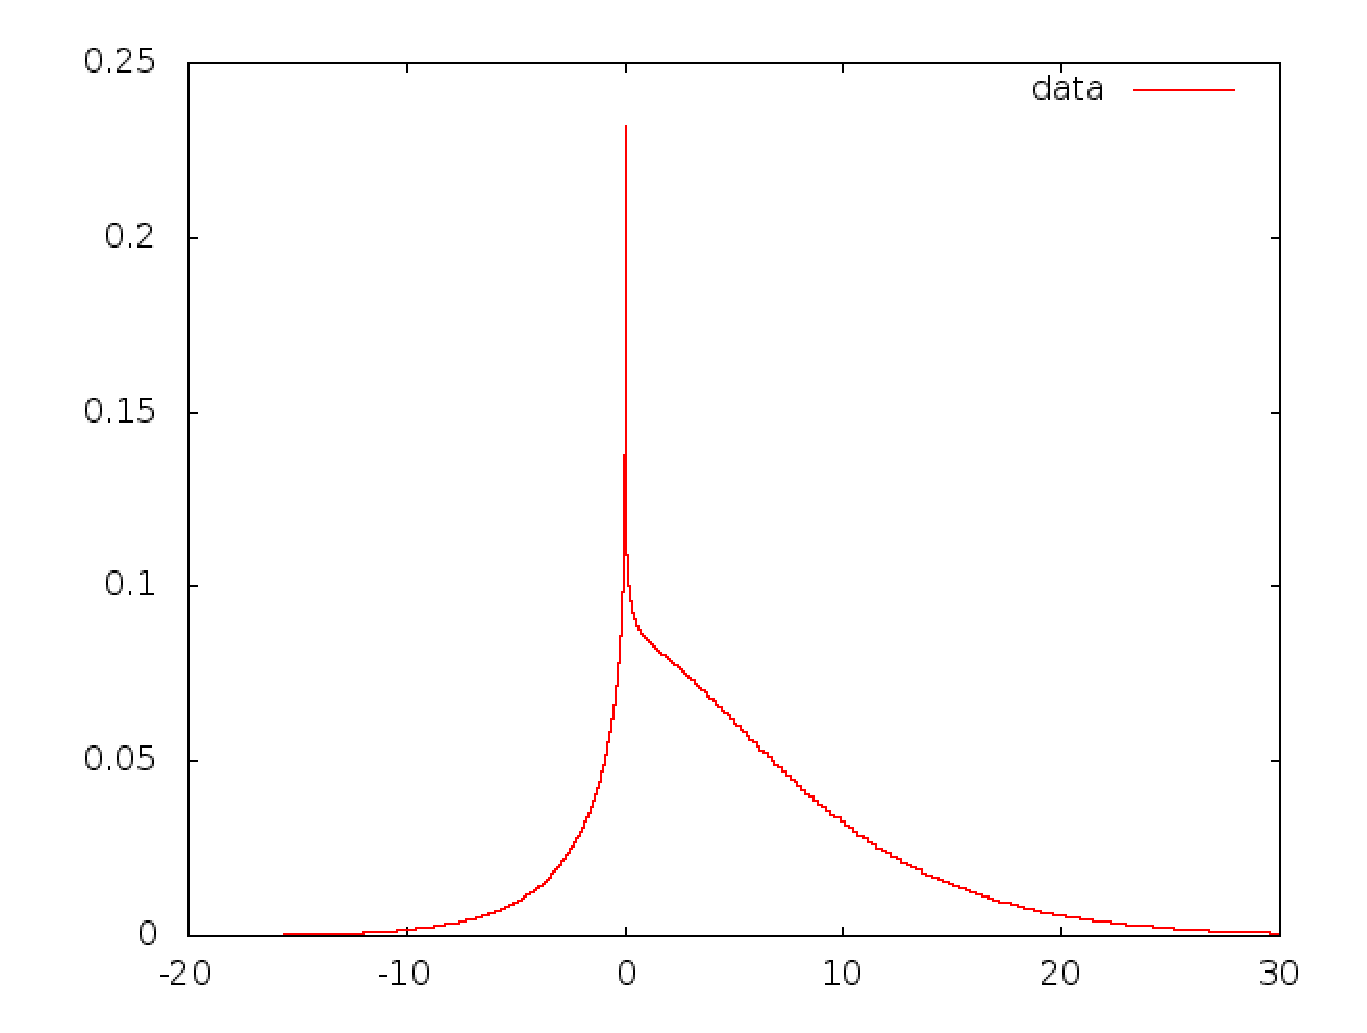
\includegraphics[width=3in]{Images/N53xN11.eps}
  \caption[N(5,3) x N(1,1)]
          {N(5,3) x N(1,1)}
  \label{fig:N53xN11}
\end{figure}

A larger example of multiplication is $XY$ where $X \sim N(5,3), Y \sim N(1,1)$. The listing follows as the plot is shown in figure \ref{fig:N53xN11}.
\begin{lstlisting}
X = Normal(5,3)
Y = Normal(1,1)
XY = X*Y
Plot().xrange(-20,30).plot(XY).show()
\end{lstlisting}

Similarly, division of two numeric random variables, this time in one line of code with the result shown in figure \ref{fig:N73_N11} which happens to be multi-modal. 
\begin{lstlisting}
Plot().xrange(-20,30).plot(Normal(7,3)/Normal(1,1)).show()
\end{lstlisting}

\begin{figure}
  \centering
  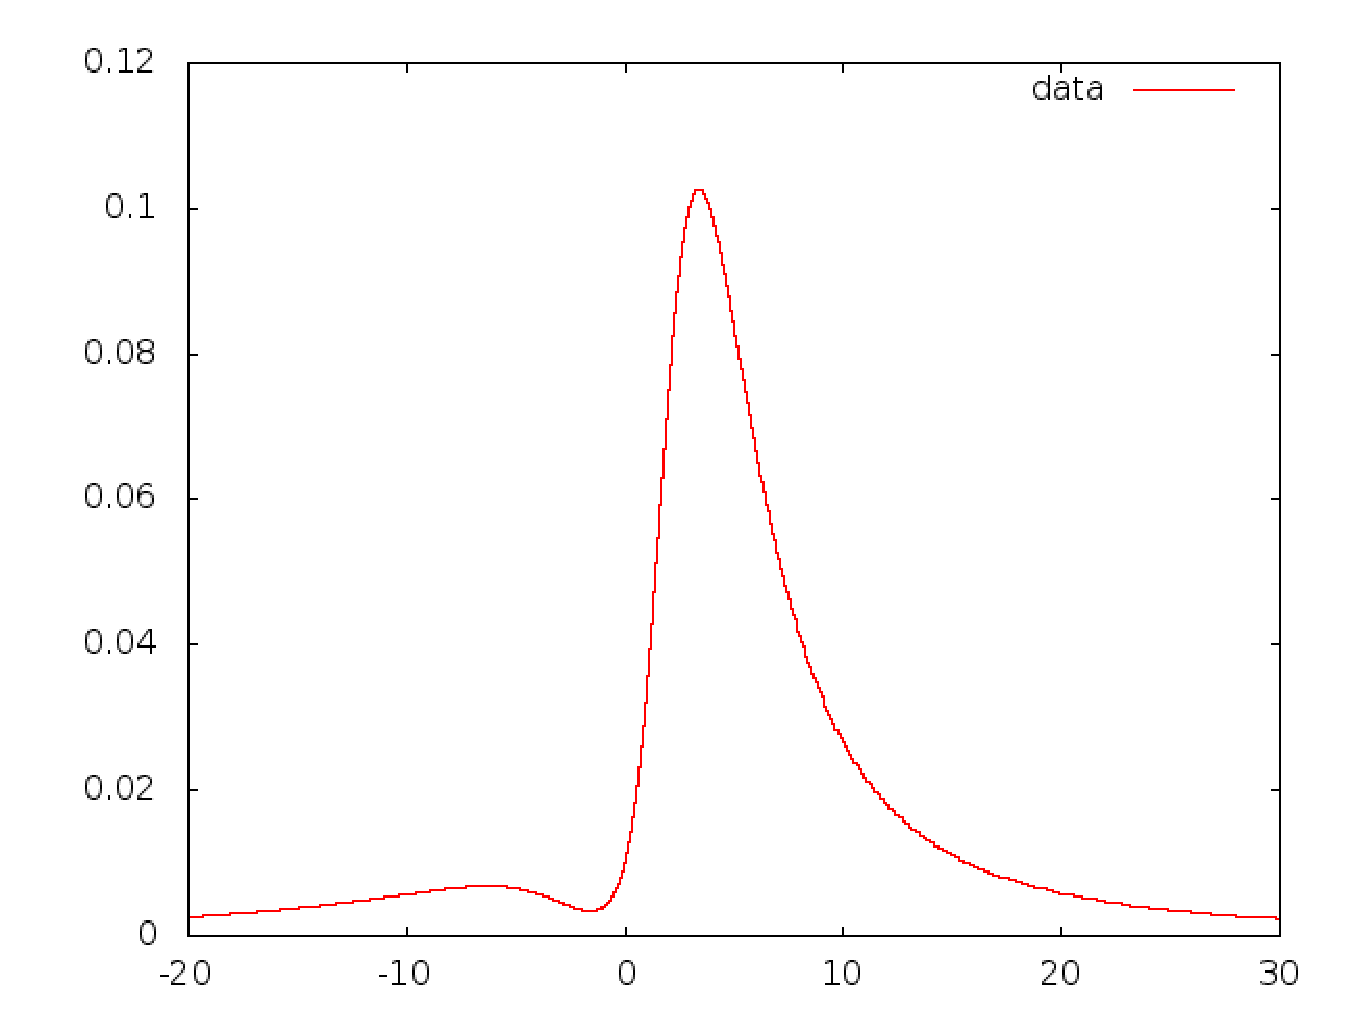
\includegraphics[width=3in]{Images/N73_N11.eps}
  \caption[N(7,3) / N(1,1)]
          {N(7,3) / N(1,1)}
  \label{fig:N73_N11}
\end{figure}

\section{Correlation}
Consider the example in figure \ref{fig:Product_Power} without preperatory remarks.
\begin{table}
\begin{center}
\begin{tabular}{cc}
$X*X$ & $X^2$\\
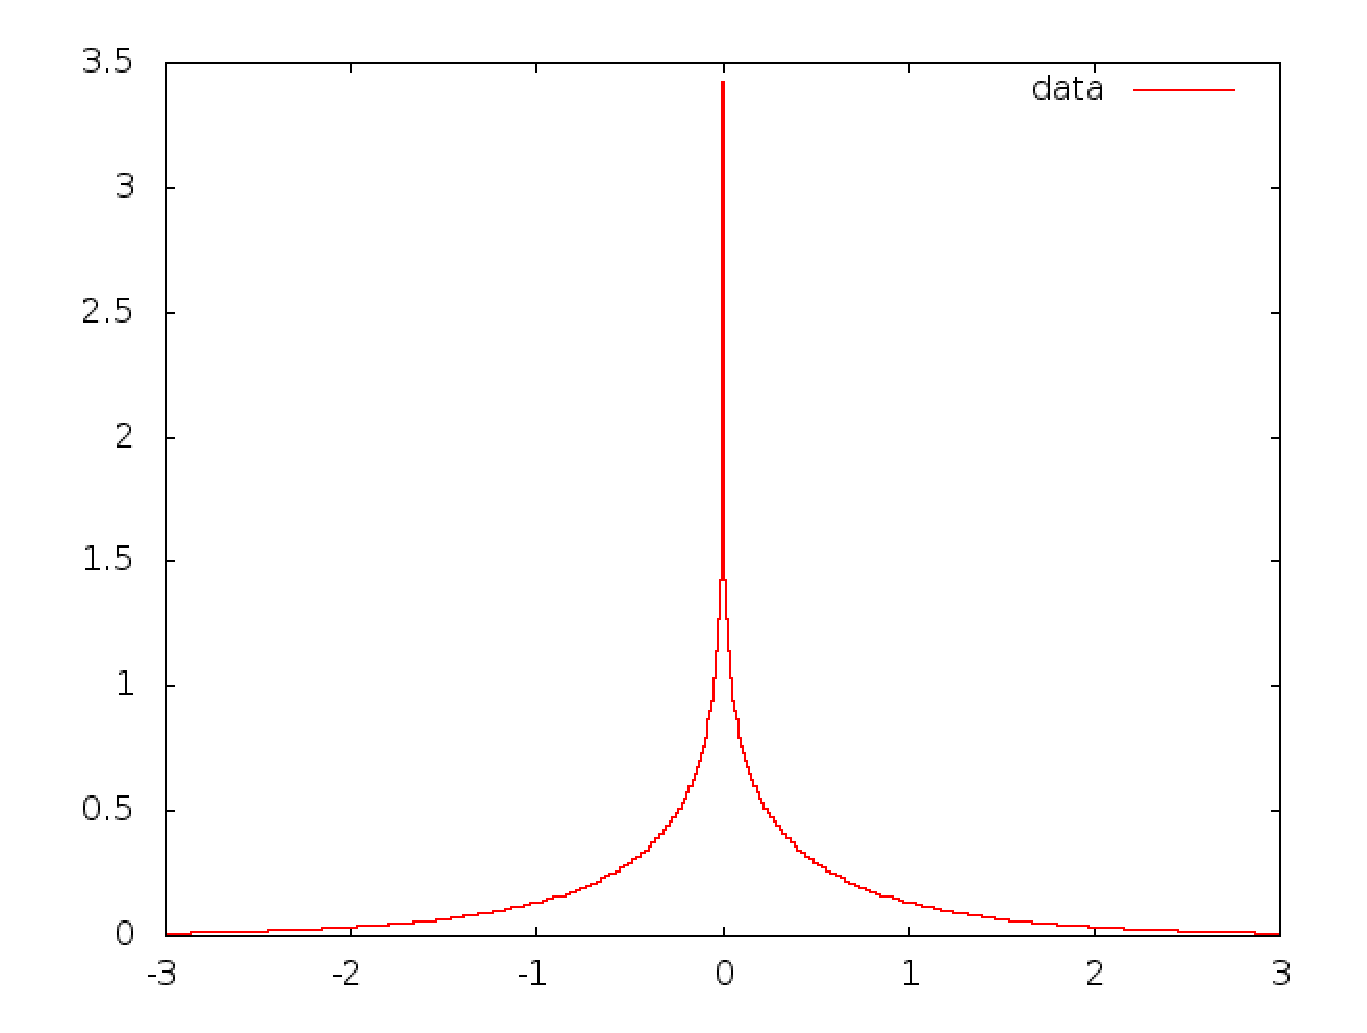
\includegraphics[width=2in]{Images/N01xN01.eps} &
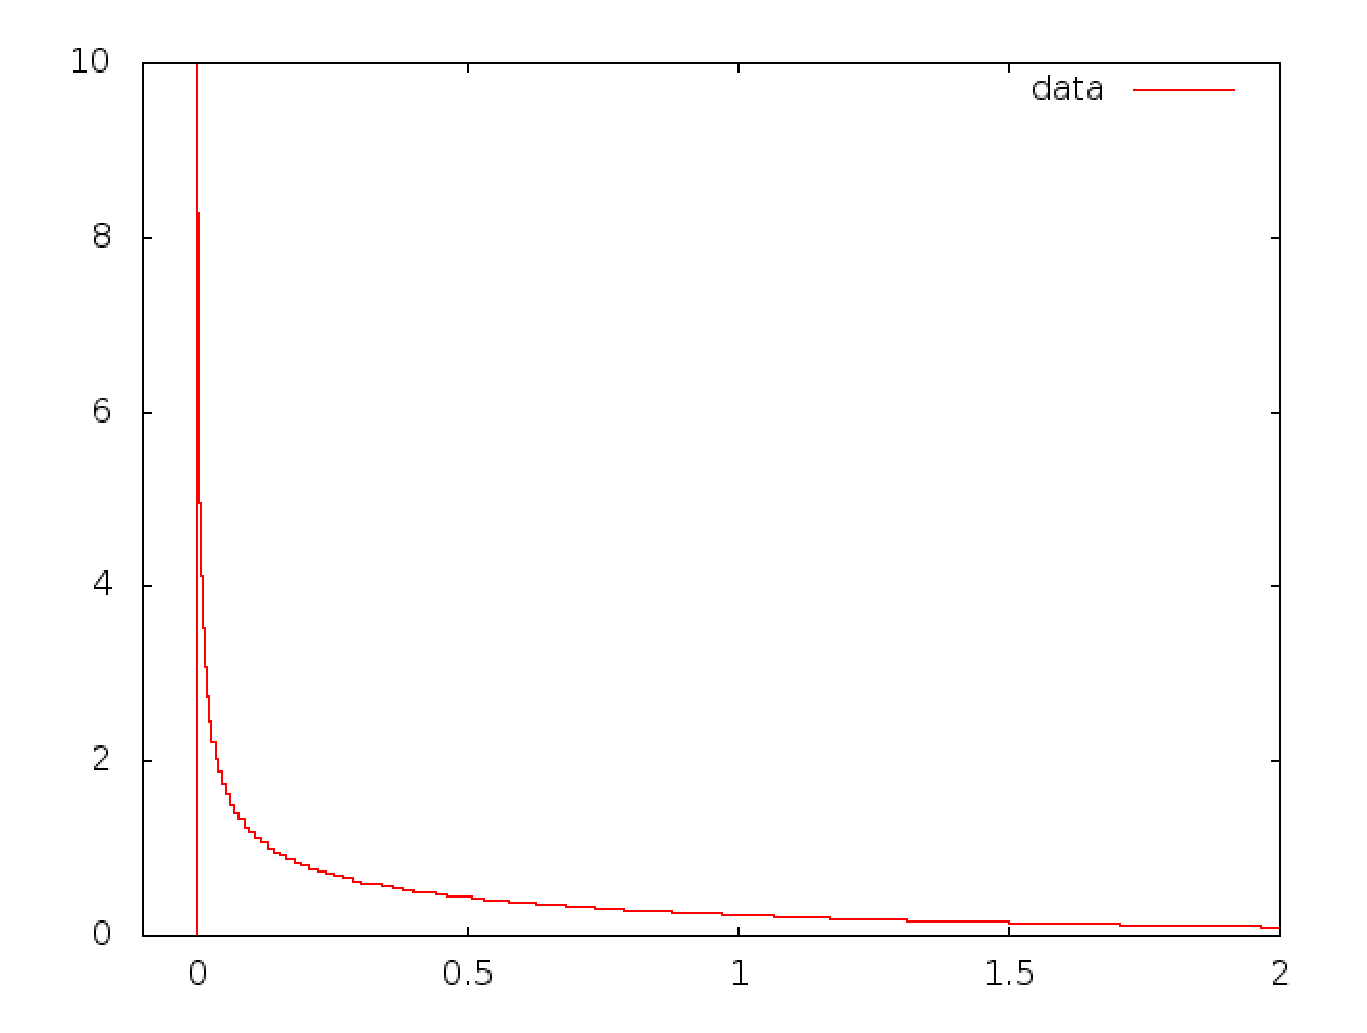
\includegraphics[width=2in]{Images/N01xx2.eps} \\
\end{tabular}
\end{center}
\caption[Standard Normal $X*X$ versus $X^2$]
        {Standard Normal $X*X$ versus $X^2$}
\label{fig:Product_Power}
\end{table}

The issue in figure \ref{fig:Product_Power} is that RICO needs to understand that two references to the same underlying variable are $100\%$ correlated. When RICO is asked to compute $X^2$ there is no confusion, but $X*X$, without correlation tracking appears as the product of two independent copies of $X$.

Within the context of an algorithmic model with some random variable inputs intermediate variables are created and mixed with other intermediate variables such that partially correlated expressions are possible,
\begin{align*}
X + XY\\
X + Y/X
\end{align*}
Assuming that $X \perp Y$ the multiplication $XY$ is between independent random variables and is computable is detailed in the previous section. The sum in $X + XY$ is not between independent random variables. Fortunately RICO is equipped with a symbolic processing engine so that the expression $X+XY$ will be factored into $X(1+Y)$. This expression is computable as a sequence of operations. The expression $1+Y$ is independent of $X$ so the product $X(1+Y)$ is between independent random variables. 

\begin{figure}
  \centering
  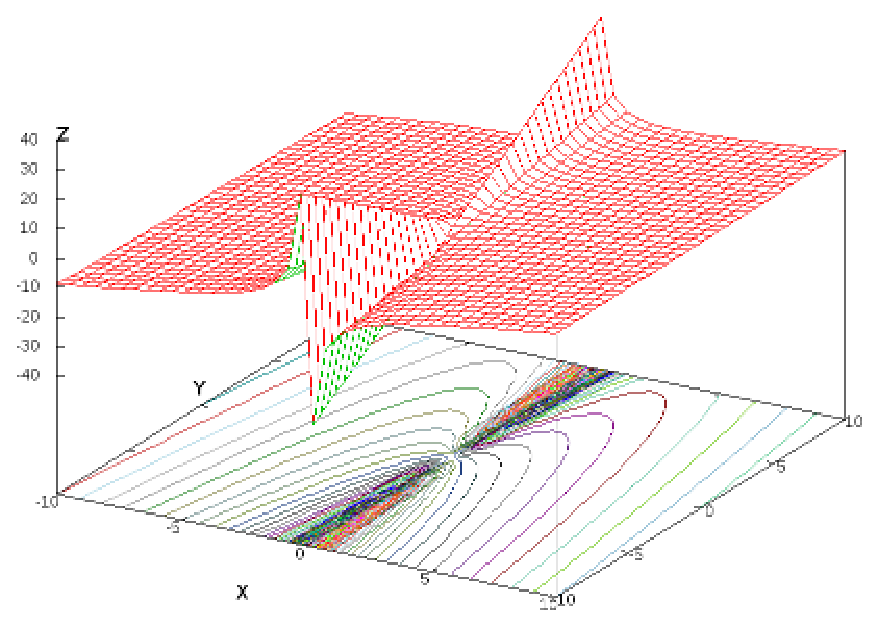
\includegraphics[width=3in]{Images/XpY_X.eps}
  \caption[X + Y/X]
          {X + Y/X}
  \label{fig:XpY_X}
\end{figure}

The expression $X+Y/X$ is not decomposible into a sequence of operations between independent random variables. In such a case the iso-probability level curves are more complicated than the hyperbolas found in the multiplication case. The level curves for a particular partition of $Z = X+Y/X$ are shown in figure \ref{fig:XpY_X}.

In the case of $Z = X + Y/X$, the partitions of $X$ and $Y$ for a partition of the joint $(X,Y)$ space. A subset of the iso-probability level curves associated with the partition of $Z$ are approximated within each $(X,Y)$-partition rectangle bounded by $(x_0, y_0)$ and $(x_1, y_1)$, relatively indexed, by approximating the supported probability surface $f$ with a bilinear function of $X$ and $Y$ as
\begin{align*}
f(x,y) = axy + bx + cy + d
\end{align*}
where the coefficients $(a,b,c,d)$ are
\begin{align*}
\begin{pmatrix}a\\b\\c\\d\end{pmatrix} = 
  \begin{pmatrix}x_0 y_0 & x_0 & y_0 & 1\\
                 x_1 y_0 & x_1 & y_0 & 1\\
                 x_0 y_1 & x_0 & y_1 & 1\\
                 x_1 y_1 & x_1 & y_1 & 1
  \end{pmatrix} ^ {-1} 
  \begin{pmatrix}
    f(x_0, y_0)\\f(x_1, y_0)\\f(x_0, y_1)\\f(x_1, y_1)
  \end{pmatrix}
\end{align*}
An iso-probability level curve is then a function $y(x | z)$ for a given partition endpoint $z$ as
\begin{align*}
y(x | z) = \frac{z - d - bx}{ax + c}
\end{align*}
A necessary step is to compute the fraction of each $(X,Y)$-partition rectangle intersected each given $Z$-partition interval. The bilinear approximation admits the following closed form solution,
\begin{align*}
\int y(x | z) \; dx = \frac{log(ax+x)(az - ad + bc)-abx}{a^2} + const
\end{align*}

\begin{figure}
  \centering
  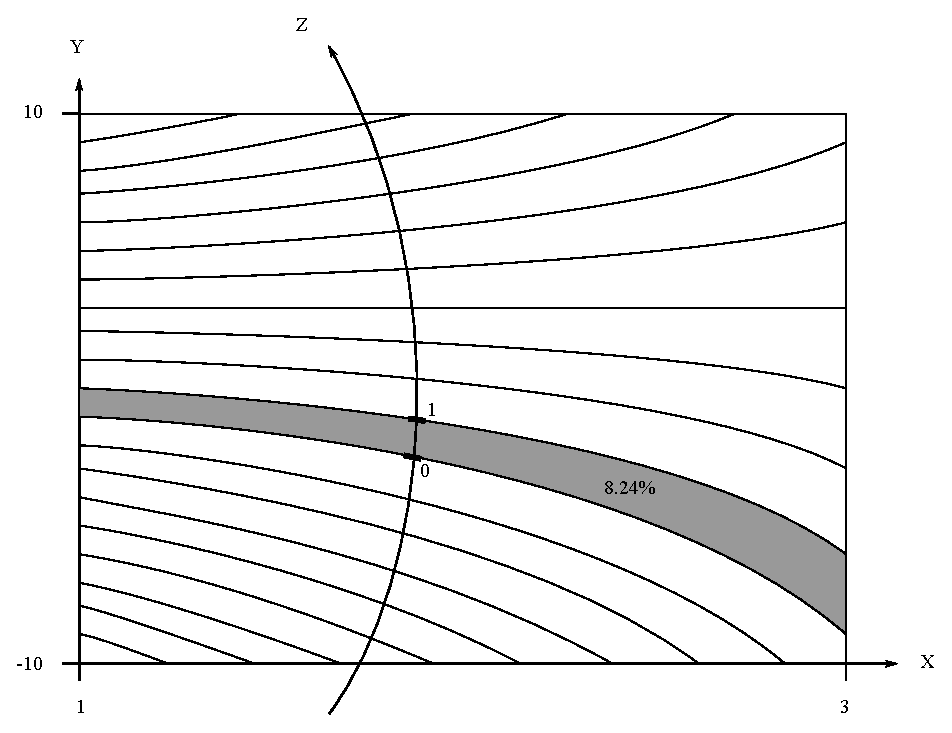
\includegraphics[width=3in]{Images/XpY_Zrectangle.eps}
  \caption[A partition element of X + Y/X with level curves]
          {A partition element of X + Y/X with level curves}
  \label{fig:XpY_Zrectangle}
\end{figure}

As a numerical example suppose $X$ has a partition element bounded by $\{1,3\}$ and similarly $Y$ has a partition element bounded by $\{-10,10\}$. If $Z$ has a partition element bounded by $\{0,1\}$ then figure \ref{fig:XpY_Zrectangle} shows that appoximately $8.25\%$ of the probability represented by this partition rectangle is allocated to the $(0,1)$ partition element of $Z$. The resulting probability distribution for $Z$ is shown in figure \ref{fig:XpY_X_Z}.

\begin{figure}
  \centering
  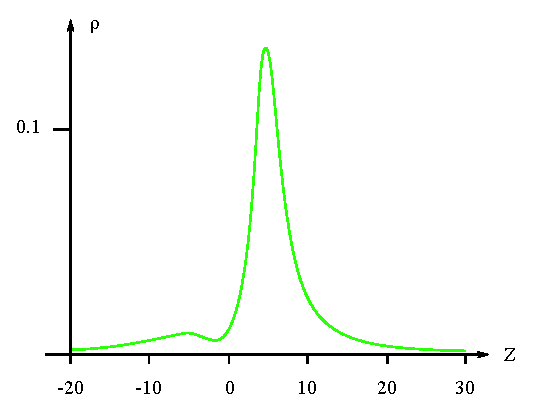
\includegraphics[width=3in]{Images/XpY_X_Z.eps}
  \caption[$X+Y/X$ where $X\sim N(5,3), Y \sim N(1,1)$]
          {$X+Y/X$ where $X\sim N(5,3), Y \sim N(1,1)$}
  \label{fig:XpY_X_Z}
\end{figure}


\chapter{Correlated Operations}
Given a random variable $A$ and two real-valued functions $f$ and $g$ such that $X = f(A)$ and $Y = g(A)$ let $Z = h(X,Y)$ where $h$ is some real-value function from $\mathbb{R}^2$. The function $h(x,y) = x+y$ is of particular interest.

Since $A$ may be a mixed random variable the development will by assuming $A$ is discrete, then continuous and finally a general mixed random variable. In all cases $X$ and $Y$ are, by design, 100\% correlated through $A$.

\subsection{Discrete Operations on Correlated Random Variables}

Suppose that,

\begin{align*}
A = ((a_1, a_2, ..., a_n), (p_1, p_2, ..., p_n))
\end{align*}

where $Pr[A = a_i] = p_i$ for any $i \in 1...n$, that is, $A$ is a discrete random variable. Consequently,

\begin{align*}
X = ((x_1, x_2, ..., x_n), (p_1, p_2, ..., p_n))\\
Y = ((y_1, y_2, ..., y_n), (p_1, p_2, ..., p_n))\\
\end{align*}

where $x_i = f(a_i)$ and $y_i = g(a_i)$  for each $i$. Notice that duplicate values of $x_i$ are possible. If it happens that $x_i < x_{i+1}$ for each $i \in 1...n-1$ then $X$ is said to be in \emph{proper form} and similarly for $A$ and $Y$. To emphasize that $X$ and $Y$ are derived in a pointwise order-preserving manner they may be written in \emph{synchronous} form,

\begin{align*}
X = (x_1, x_2, ..., x_n)\\
Y = (y_1, y_2, ..., y_n)
\end{align*}

where the probability values associated with each $x_i$ and $y_i$ are found in $A$. The joint probability distribution of $X$ and $Y$ is itself a random variable called $XY$. Stated in syncrhonous form,

\begin{align*}
XY = ((x_1, y_1), (x_2, y_2), ..., (x_n, y_n))
\end{align*}

A new random variable $Z = h(X,Y)$ is stated in synchronous form with respect to $A$ as,

\begin{align*}
Z &= (h(x_1, y_1), h(x_2, y_2), ..., h(x_n, y_n))
\end{align*}

To restate $Z$ in proper form requires two steps. The first is to remove duplicates form the range of $Z$,

\begin{align*}
\mathbf{R}(Z) = \{h(x_i, y_i)\}_{i \in 1..n}
\end{align*}

The second step is to find the probability associated with each element of the range of $Z$. Assuming the following proper form of $Z$ as,

\begin{align*}
Z = ((z_1, z_2, ..., z_m), (q_1, q_2, ..., q_m))
\end{align*}

where $m \le n$ then,

\begin{align*}
z_j &\in \mathbf{R}(Z) \text{, ordered ascending}\\
q_j &= \sum_{i | z_j = h(x_i, y_i)}p_i
\end{align*}

For example suppose,

\begin{align*}
A = ((a_1,a_2,a_3),(p_1,p_2,p_3))\\
X = (1,2,3)\\
Y = (1,3,2)
\end{align*}

The joint random variable $XY$ in synchronous form is,

\begin{align*}
XY = ((1,1), (2,3),(3,2))
\end{align*}

Suppose $Z = h(X,Y)$ where $h(x,y) = x+y$. Then $Z$ in synchronous form with respect to $A$ is,

\begin{align*}
Z = (2, 5, 5)
\end{align*}

To find the proper form of $Z$ the range is first determined,

\begin{align*}
\mathbf{R}(Z) = \{2,5\}
\end{align*}

the proper form of $Z$ is stated as,

\begin{align*}
Z = ((z_1, z_2), (q_1, q_2))
\end{align*}

where

\begin{align*}
q_1 &= p_1\\
q_2 &= p_2 + p_3
\end{align*}

since $Z = 5$ is the set $\{(x_2,y_2) = (2,3), (x_3, y_3) = (3,2)\}$. Notice that the process of finding $Z$ in proper form is that of integrating iso-value subsets of the joint $XY$ range, the domain of $Z$. 

\subsection{Continous Operations on Correlated Random Variables}

Suppose $A$ is a real-valued continous random variable. Let $P$ be the probability density function associate with $A$ and write $A \sim P$. The random variables $X = f(A)$ and $Y = g(A)$, in synchronous form, share this association with $A$, that is, $X ~ P$ and $Y ~ P$ for any real valued functions $f$ and $g$. The joint random variable $XY$ is also stated in synchronous form as $XY \sim P$. Finally, $Z = h(XY)$ for any real-valued function $h$ from $\mathbb{R}^2$ is also stated in synchronous form as $Z \sim P$. 

To form an interesting example consider that $X = f(A)$ and $Y = g(A)$ form a parametric curve in $XY$-space and that the probability density $P$ is distributed along this curve. If $Z = h(XY)$ such that $h(x,y) = x+y$ then iso-value contours in $XY$-space appear as parallel lines with slope $-1$. In the figure \ref{fig:XY_continous} the disjoint curves are the single parametric $(X,Y)$ curve and the dotted diagonal lines are the iso-value contours for addition of $X$ and $Y$. The probability density $P$ of $A$ would appear in the figure perpendicular to the $XY$ plane over the paremetric curve of $(X,Y$). From the figure it is apparent that $Pr(1 < Z < 5) = 1$. Notice that the iso-value contour labeled $5$ in the figure intersects the $XY$ curve at three places so that $Pr(Z = 4)$ is found as the sum of three probability density values in $P$. 

\begin{figure}
  \centering
  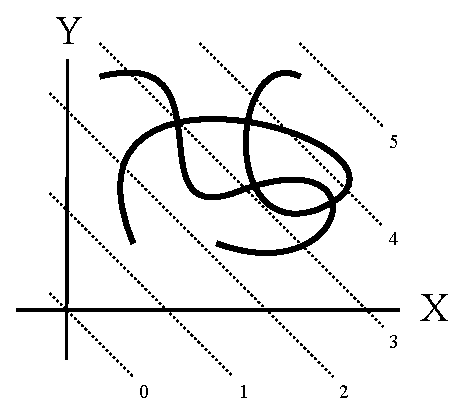
\includegraphics{Images/XY_continous.eps}
  \caption[Joint distribution of correlated Continuous $X$ and $Y$ in $XY$-space]
          {Distribution of Continuous $XY$}
  \label{fig:XY_continous}
\end{figure}

Stating the synchronous form of $Z$ with respect to $A$ is as simple as for $X$ and $Y$, that is, $Z \sim P$. Finding the proper form of $Z$ may be a more challenging problem. The procedure for computing a numerical approximation to the proper form of $Z$ is detailed in the dissertation \cite{fielden12}. Notice in particular that computing the proper form of a random variable may be avoided until and observation is required for reasons such as graphing or comparison to unrelated random variables and constant values.

\subsection{Mixed Discrete / Continuous Operations on Correlated Random Variables}

To prepare for the computation of operations on a pair of mixed discrete/continuous random variables dependent on a single common random variable, it is useful to develop the case where one operand is discrete and the other is continuous. This situation can only arise if $A$ is not a purely discrete random variable.

Suppose that $A$ is a continuous random variable such that $A \sim P$ as above. Suppose without loss of generality that $X$ is a discrete random variable and that $Y$ is a continuous random variable. A visual example of a possible joint random variable $XY$ appears in figure \ref{fig:XY_discrete_continuous}. Included in the figure are the iso-value contours used to compute $Z = h(XY)$ where $h(x,y) = x+y$ as the previous continous example. Notice that this case is not fundamentally different from the previous case where $X$ and $Y$ are both continous. In the figure $X$ has four unique values in its range labeled $x_1, x_2, x_3, x_4$. It is apparent from the figure that $Pr(1 < Z < 5) = 1$ and that $Z$ is a continuous random variable. The procedure for computing a numerical approximation to the proper form of $Z$ is detailed in the dissertation \cite{fielden12}. 

\begin{figure}
  \centering
  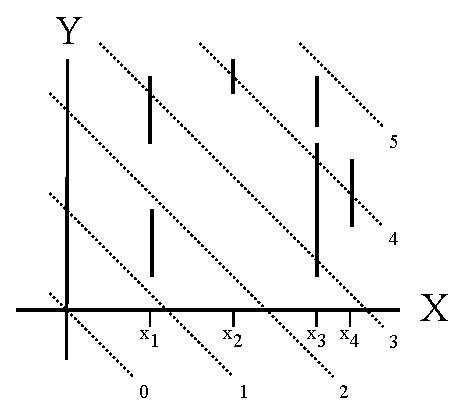
\includegraphics{Images/XY_discrete_continous.eps}
  \caption[Joint Distribution of Correlated Discrete $X$ and Continous $Y$ in $XY$-space]
          {Distribution of Discrete/Continous $XY$}
  \label{fig:XY_discrete_continuous}
\end{figure}

\subsection{Operations on Correlated Mixed Random Variables}

If random variable $A$ is \emph{mixed}, that is, containing both continous and discrete probability distributions it is useful to decompose it into discrete and continous components and write,

\begin{align*}
A = A_d \oplus A_c
\end{align*}

where $A_d$ is a discrete random variable and $A_c$ is a continuous random variable and the $'\oplus'$ operator performs a sum of distribution functions by converting discrete probability to Dirac Delta functions. The components of $A$ are written as,

\begin{align*}
A_d &= ((a_1, ..., a_n),(p_1, ..., p_n))\\
A_c &\sim Q
\end{align*}

where $Q$ is a conditional probability distribution represented by a continuous probability density function. Notice that if $d = Pr(A_d)$ then $Pr(A_c) = 1-d$. That is,

\begin{align*}
d &= \sum_{i = 1..n}p_i\\
1-d &= \int_{A_c} dQ
\end{align*}

where the abuse of integral notation implies that the integral is performed over the range of $A_c$ in the usual sense. A non-trivial mixed random variable then requires that $0 < d < 1$. 

Notice in particular that for special case of addition of correlated random variables the operation of addition as in $Z = X+Y$ is that of projecting the $XY$ distribution to the diagonal as shown in figure \ref{fig:XY_addition_projection}. 

\begin{figure}
  \centering
  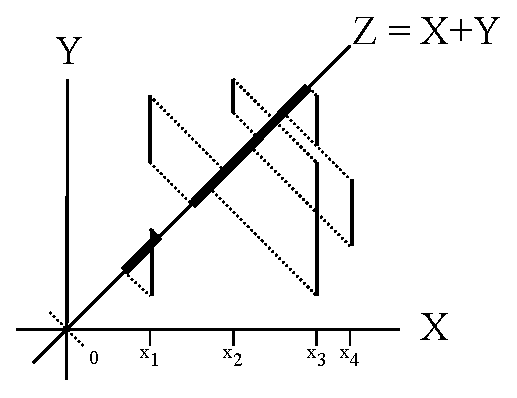
\includegraphics{Images/XY_addition_projection.eps}
  \caption[Projection of $XY$-space to $X+Y$-space]
          {Projection of $XY$-space to $X+Y$-space}
  \label{fig:XY_addition_projection}
\end{figure}

As an example suppose,

\begin{align*}
A &= \mathbf{U}(-1,2)\\
f(x) &= step(x) = \begin{cases}
0 & \text{ if x $\le$ 0},\\
1 & \text{ else}
\end{cases}\\
g(y) &= |y| + 1\\
X &= f(A)\\
Y &= g(A)
\end{align*}

then in proper form,

\begin{align*}
X &= ((0,1),(\frac{1}{3},\frac{2}{3}))\\
Y &= \mathbf{U}((0,1,2),(\frac{2}{3}, \frac{1}{3}))
\end{align*}

where $Y$ is \emph{multi-uniform} requiring probabilities within partition elements to be specified. Notice that $Pr(X = 0) = \frac{1}{3}$, $Pr(X = 1) = \frac{2}{3}$, $Pr(0 < Y < 1) = \frac{2}{3}$ and $Pr(1 < Y < 2) = \frac{1}{3}$. 

Suppose further that $Z = X+Y$. The joint $XY$ figure \ref{fig:XY_01_example} reveals the details. Noticing that the probability is uniformly distributed over the range of $XY$ and that the two fragments of that region do not overlap according to the iso-value contours of $Z$ the problem is solved by inspection so that,

\begin{align*}
Z \sim \mathbf{U}(1,4)
\end{align*}

\begin{figure}
  \centering
  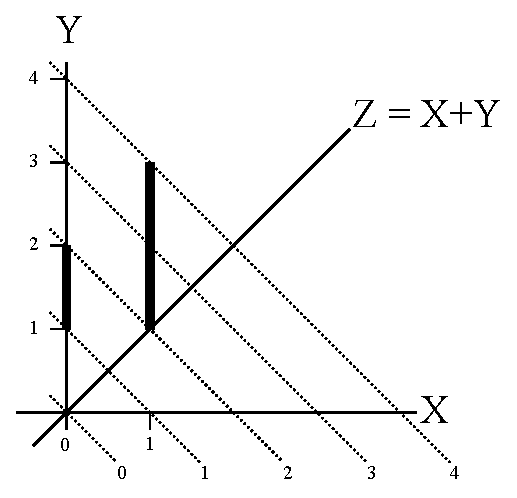
\includegraphics{Images/XY_01_example.eps}
  \caption[Example of Correlated Discrete $X$ and Continous $Y$ in $XY$-space]
          {Example of Discrete/Continous $XY$}
  \label{fig:XY_01_example}
\end{figure}

To find this result more formally $Y$ is conditioned on the discrete $X$ so that,

\begin{align*}
Y | X = 0 &\sim \mathbb{U}(1,2)\\
Y | X = 1 &\sim \mathbb{U}(1,3)
\end{align*}

then,

\begin{align*}
Z &= X + Y\\
  &= (X + Y | X = 0) \oplus (X + Y | X = 1)\\
  &= (0 + Y | X = 0) \oplus (1 + Y | X = 1)\\
  &\sim \mathbf{U}(1+0,2+0) * Pr(X = 0) + \mathbf{U}(1+1,3+1) * Pr(X = 1)\\
  &\sim \mathbf{U}(1,2) * \frac{1}{3} + \mathbf{U}(2,4) * \frac{2}{3}\\
  &\sim \mathbf{U}(1,4)
\end{align*}

For visual convenience the proper form distributions of $A$, $X$, $Y$ and $Z$ are shown in figure \ref{fig:XY_example_distributions}. Notice that to compute $Z = X + Y$ from the proper forms of $X$ and $Y$ is more challenging than from the synchronous form of $XY$ in figure \ref{fig:XY_01_example} in part because of the otherwise unseen correlation between $X$ and $Y$ through $A$.

\begin{figure}
  \centering
  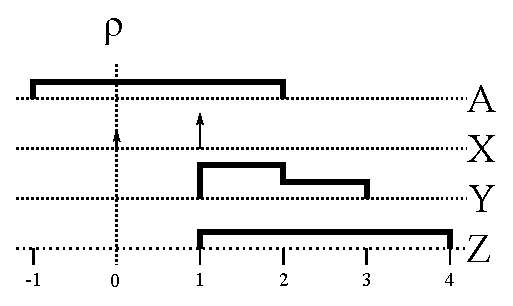
\includegraphics{Images/XY_example_distributions.eps}
  \caption[Example Discrete/Continuous Distributions in Proper Form]
          {Example Discrete/Continous Distributions in Proper Form}
  \label{fig:XY_example_distributions}
\end{figure}

\chapter{Constrained Optimization}
\section{Tables and Chairs with Correlated Random Prices}

In this final stage of the tables and chairs example consider correlated random prices. Common practice when writing about economic matters is to develop a story around the problem to help tie the elements together. This practice will be followed for this example.

Suppose that a small furniture manufacturer in Portland, Oregon wants to forecast weekly revenue. The manufacturer makes tables and chairs in a small show with a small crew. Using a forecast for demand for tables, chairs and dinette sets the manufacturer derives the likely market prices for tables and chairs. A dinette set is composed of one table and two chairs.

Figure \ref{fig:TCD} shows the independent random variables corresponding to forecast demand for dinette sets (the exponential curve), tables (the tall Gaussian curve) and chairs (the wide Chi-Squared curve). The vertical axis represents probability density and the horizontal axis represents demand for units (in thousands) in the Portland market.

\begin{figure}
  \centering
  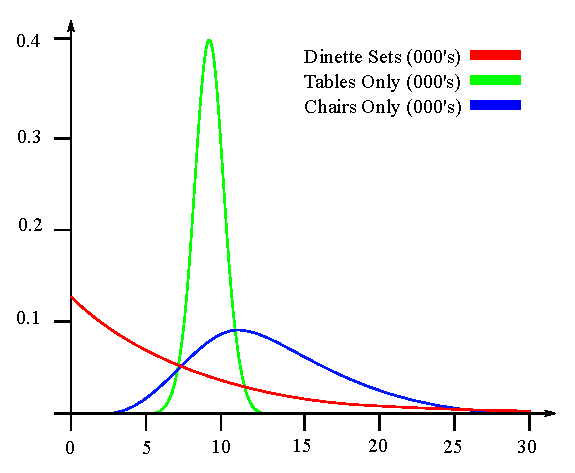
\includegraphics[width=120mm]{Images/TCD}
  \caption[Tables, Chairs and Dinette Sets Random Variables]
          {Tables, Chairs and Dinette Sets Random Variables}
  \label{fig:TCD}
\end{figure}

The manufacturer believes that market price and demand for tables are related by the inverse function,

\begin{align*}
P_t = \frac{14*80}{D_t + D_d}
\end{align*}

where $D_t$ is the demand for tables alone and $D_d$ is the demand for dinette sets. Thus $D_t + D_d$ is the total demand for tables. Similarly, the price of chairs is related to the demand for chairs by the inverse function,

\begin{align*}
P_c = \frac{24*45}{D_c + 2D_d}
\end{align*}

where $D_c$ is the demand for chairs alone and again $D_d$ is the demand for dinette sets. The sale of one dinette set implies the sale of two chairs. The actual functions are immaterial and have been contrived so that the results of this version of the tables and chairs example are comparable to previous versions. 

Recognize that $P_t$ and $P_c$ are correlated, but do not need to materialize their joint probability distribution in order to compute revenue results.

The example is data-intensive and prototype software is used to produce numerical results. Rather than presenting the prototype, written in Python using the Numpy library, the data structures and sequence of operations will be described.

Let the input random variables be,

\begin{align*}
Dt &= \{DXt, DPt\}\\
Dc &= \{DXc, DPc\}\\
Dd &= \{DXd, DPd\}
\end{align*}

where,

\begin{align*}
DXt &= (DXt_1, \dots, DXt_{Nt})\\
DPt &= (DPt_1, \dots, DPt_{Nt})\\
DXc &= (DXc_1, \dots, DXc_{Nc})\\
DPc &= (DPc_1, \dots, DPc_{Nc})\\
DXd &= (DXd_1, \dots, DXd_{Nd})\\
DPd &= (DPd_1, \dots, DPd_{Nd})
\end{align*}

assuming that $DPt_{Nt} = DPc_{Nc} = DPd_{Nd} = 0$ as usual for the numeric random variables since probability values are between partition values. Then $Nt$, $Nc$ and $Nd$ as the number of partition endpoints for each input random variable; tables, chairs and dinette sets respectively.

Form the demand joint probability distribution $DP$ for the input random variables by Cartesian product,

\begin{align*}
DP &= DPt \times DPc \times DPd
\end{align*}

Separately form parallel 3D arrays for each input demand,

\begin{align*}
DT &= DXt \times ones(Nc) \times ones(Nd)\\
DC &= ones(Nt) \times DXc \times ones(Nd)\\
DD &= ones(Nt) \times ones(Nc) \times DXd
\end{align*}

where, defining by example,

\begin{align*}
ones(5) = (1, 1, 1, 1, 1)
\end{align*}

Throughout this example presentation 2D diagrams will tend to be preferred to represent 3D objects for clarity. In figure \ref{fig:tcd_rectangle} the demand joint probability $DP$ is represented for a fixed value of $DXd$.

\begin{figure}
  \centering
  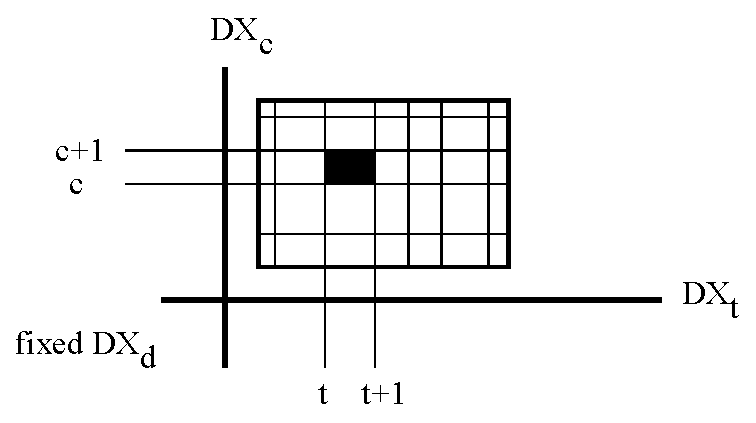
\includegraphics{Images/tcd_rectangle}
  \caption[One Layer of Demand Probability Array]
          {One Layer of Demand Probability Array}
  \label{fig:tcd_rectangle}
\end{figure}

In an abuse of notation, when no confusion arises, $t$, $c$ and $d$ are used as both identifiers and indices. The indices for tables, chairs and dinette set random variables are,

\begin{align*}
t &= 1 \dots Nt\\
c &= 1 \dots Nc\\
d &= 1 \dots Nd
\end{align*}

A specific point will be referred to within the demand joint probability array as $DP_{t,c,d}$ or simply $DP_{tcd}$ where the commas are dropped for clarity. The shaded rectangle in figure \ref{fig:tcd_rectangle} is then the demand-space rectangular block of uniform probability distribution with value $DP_{tcd}$.

The four 3D arrays $DT$, $DC$, $DD$ and $DP$ are all parallel. Create other arrays parallel to these. The reason for this parallelism is to ensure that the probability within each block is correctly tracked through each step of the computation process.

The 3D arrays for the prices of tables and chairs are then written,

\begin{align*}
PT &= \frac{14*80}{DT + DD}\\
PC &= \frac{24*45}{DC + 2 DD}
\end{align*}

where the sums, $DT+DD$ and $DC + 2DD$, are computed element-wise as well as the reciprocal functions. The result is that $PT$ and $PC$ are 3D arrays of size $Nt*Nc*Nd$ and are parallel to the demand and demand probability arrays. Note in particular that the price arrays $PT$ and $PC$ are not random variables. They may be converted to random variable form as detailed below. This is possible because values of prices are located at vertices of a block of probability distribution and the value of the probability is uniformly distributed within that block in the 3D array $DP$.

Now that input prices are established for the manufacturer optimization may be applied to decide what combination of tables and chairs to produce. In this example the optimization is computed exhaustively and the demand space is readily paritioned into three output cases $A$, $B$ and $C$. 

Consider that each point in the 3D demand array represents a particular choice of input values that has associated with it two particular prices, one for tables and the other for chairs. It is known, for example, that if $\frac{2}{3}Pt < Pc$ then output $A$ will be selected and similar rules apply for outputs $B$ and $C$. This means that for each point in the 3D demand space a Boolean value $1$ or $0$ can be assigned where $1$ means that point has an associated price for chairs that is larger then two-thirds that of tables. A parallel 3D array of Boolean values called a \emph{mask} based on the optimized output selection rules results. Let,

\begin{align*}
MA &= \frac{2}{3}PT < PC\\
MB &= \frac{1}{4}PT < PC < \frac{2}{3}PT\\
MC &= PC < \frac{1}{4}PT
\end{align*}

Each output is associated with some revenue. Using the price arrays, parallel revenue arrays may be formed. Let,

\begin{align*}
RA &= 45PC\\
RB &= 24PC + 14PT\\
RC &= 20PT
\end{align*}

To convert  the revenue arrays, $RA$, $RB$ and $RC$ into random variables a partition must be identified. Noticing that while the revenue arrays are parallel, the masks indicate that any given point in the array space indexed by $(t,c,d)$ is intended to be present in exactly one revenue array. This is because the output $A$, $B$ and $C$ are mutually exclusive so, for example, the probability of producing \$1000 and \$2000 of revenue using output $A$ can be added to the probability of producing this same range of revenue for output $B$ and for $C$ to arrive at a probability of producing that range of revenue regardless of output choice. 

The partition used for the revenue random variable must span the range of possible revenue values and be fine where there is more revenue information and course where there is less and be so fine overall that numerical artifacts do not overwhelm the result. In this example every $23^rd$ point from each $175$-point input demand random variable is chosen and the problem rerun on the partition values alone, not the probability values. In the Python code this amounts to a single function call since all the code is in place for the main computation. The result is are smaller versions over the same revenue arrays representing collectively a sample of the possible revenue values this example model produces using the given demand inputs. The steps are as follows,

\begin{enumerate}
\item Form one dimensional arrays of valid revenue values for each output.
\item Run the same process as above to generate revenue arrays and output masks. Prepend an $s$ to the name indicating they are small versions due to the reduced partition size.
\item Concatenate the three 1D arrays into a single array called $temp$.
\item Sort the $temporary$ array and remove any duplicates.
\item append the value $-\infty$ to the start of the array and $\infty$ to the end. Call the result $Rx$.
\end{enumerate}

In this case the Python code from the prototype sums up the process concisely,

\begin{align*}
temp &= concatenate((sRA[sMA], sRB[sMB], sRC[sMC]))\\
Rx &= concatenate(([-\infty], unique(temp), [+\infty]))
\end{align*}

where $sRA[sMA]$ returns a one dimensional array from an arbitrary array only for points where the corresponding point in the $sMA$ small output mask array is a $1$ and $unique()$ sorts and removes duplicates from an array. 

For each (big) output array $RA$, $RB$ and $RC$ with associated masks $MA$, $MB$ and $MC$ a one dimensional array is created for the probability distribution that is parallel to the one dimensional partition array $Rx$. 

\begin{align*}
Rap &= zeros(Rx)\\
Rbp &= zeros(Rx)\\
Rcp &= zeros(Rx)
\end{align*}

where, defining by example,

\begin{align*}
zeros(5) = (0, 0, 0, 0, 0)
\end{align*}

The probability arrays, once filled in, will complete the formation of the output revenue random variables,

\begin{align*}
Ra &= \{Rx, Rap\}\\
Rb &= \{Rx, Rbp\}\\
Rc &= \{Rx, Rcp\}
\end{align*}

The three output random variables $Ra$, $Rb$ and $Rc$ are mutually exclusive and since they share a common partition their probability values are summable to find the final output revenue random variable $R$,

\begin{align*}
R = \{Rx, Rap + Rbp + Rcp\}
\end{align*}

It remains to describe how to fill in the probability arrays $Rap$, $Rbp$ and $Rcp$. The process for $Rap$ is the same for the others.

Given the (big) output revenue 3D array $RA$, its associated mask $MA$, the associated 3D probability array $DP$ and the 1D revenue partition $Rx$ the zero-valued 1D probability array $Rap$ may be created using the following steps. 

The output revenue 3D array $RA$ together with the associated probability array $DP$ describes a partition of the joint demand (input) space into blocks. Recall that the blocks have indices $t$,$c$ and $d$ so that the $(t,c,d)$ block has uniform probability $DP_{tcd}$ and eight vertices with the following revenues,

\begin{align*}
RA_{t,c,d} && RA_{t,c,d+1} && RA_{t,c+1,d} && RA_{t,c+1,d+1}\\
RA_{t+1,c,d} && RA_{t+1,c,d+1} && RA_{t+1,c+1,d} && RA_{t+1,c+1,d+1}
\end{align*}

for some block such that $1 \le t < Nt$, $1 \le c < Nc$ and $1 \le d < Nd$. If all the vertices are \emph{valid}, that is, the associated mask value is $1$ for each vertex then figure \ref{fig:block_projection} symbolically represents one possible scenario.

\begin{figure}
  \centering
  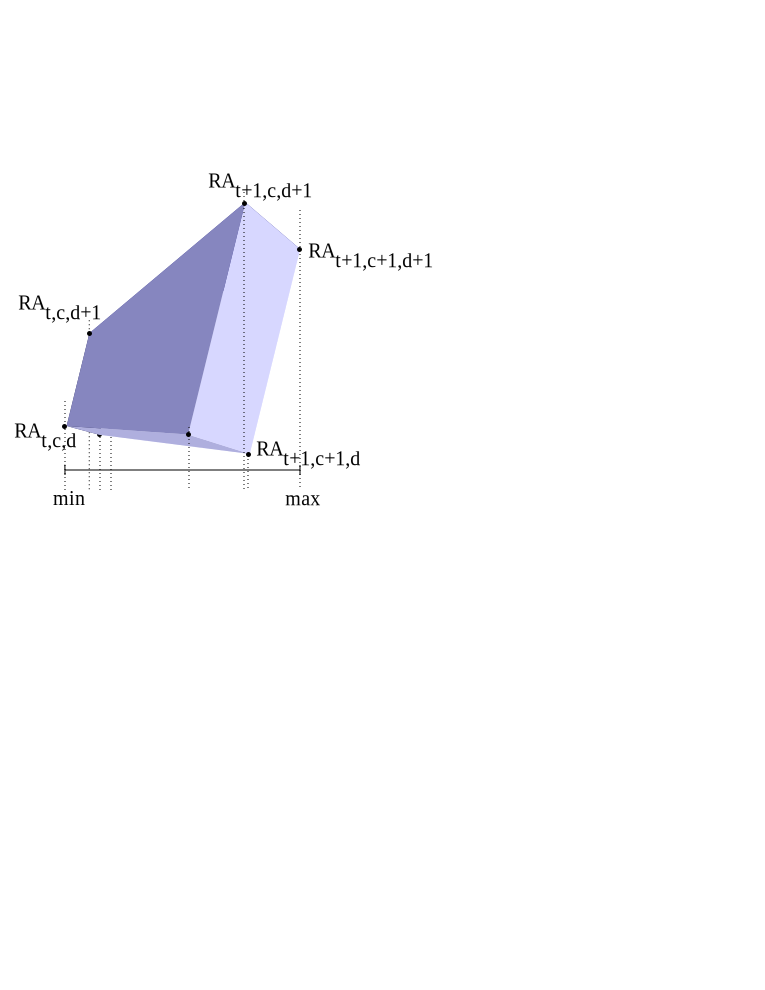
\includegraphics[width=3in]{Images/block_projection}
  \caption[Line Projection of 3D Probability Block]
          {Line Projection of 3D Probability Block}
  \label{fig:block_projection}
\end{figure}

The limits of the 3D block projection are the minimum and maximum revenue vertex values. That is,

\begin{align*}
min_{tcd} &= Min(RA_{t,c,d}, \dots, RA_{t+1,c+1,d+1})\\
max_{tcd} &= Max(RA_{t,c,d}, \dots, RA_{t+1,c+1,d+1})
\end{align*}

For the software prototype version of this example it is assumed that the 3D block probability $DP_{t,c,d}$ is distributed uniformly over the revenue line segment $(min, max)$ so that the density is $h_{tcd}$,

\begin{align*}
h_{tcd} = \frac{DP_{tcd}}{max_{tcd} - max_{tcd}}
\end{align*}

where it is assumed that $min_{tcd} < max_{tcd}$. The special cases when $min_{tcd}$ and $max_{tcd}$ are equal will be detailed below. Continuing with the general case the uniform probability density $h_{tcd}$ is allocated to the revenue probability array $Rap$ recalling that $Rap$ is delimited by the partition array $Rx$. Referring to figure \ref{fig:line_projection},

\begin{figure}
  \centering
  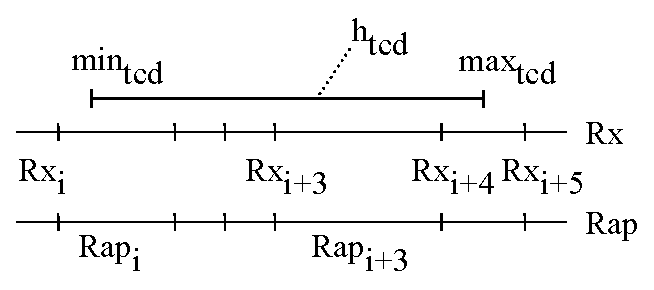
\includegraphics[width=3in]{Images/line_projection}
  \caption[Partition Allocation of Probability Line]
          {Partition Allocation of Probability Line}
  \label{fig:line_projection}
\end{figure}

\begin{align*}
Rap_i &= Rap_i + (Rx_{i+1} - min_{tcd}) h_{tcd}\\
\dots\\
Rap_{i+3} &= Rap_{i+3} + (Rx_{i+4} - Rx_{i+3}) h_{tcd}\\
Rap_{i+4} &= Rap_{i+4} + (max_{tcd} - Rx_{i+4}) h_{tcd} 
\end{align*}

where it is indicated how to compute end cases as well as cases where $Rx$ partitions are spanned by the $(min_{tcd}, max_{tcd})$ interval. 

If the mask $MA$ indicates that some of the vertices of the $(t,c,d)$ block are not valid then the amount of block probability $DP_{tcd}$ available for allocation must be reduced. For example, if $3$ of $8$ vertices are valid for the $(t,c,d)$ block then the block probability is correspondingly reduced to $\frac{3}{8}DP_{tcd}$ so that the $(min_{tcd}, max_{tcd})$ interval probability density is,

\begin{align*}
h_{tcd} = \frac{3}{8}\frac{DP_{tcd}}{max_{tcd} - max_{tcd}}
\end{align*}

If it happened that $min_{tcd} = max_{tcd}$ either because all the valid vertices have the same revenue value or there is only one valid vertex for the $(t,c,d)$ block then the corresponding partition element is located for the $Rap$ array and its value is incremented with the available probability for that block. If it happens that $min_{tcd} = max_{tcd}$ equals an $Rx$ partition endpoint then the available block probability is halved and allocated to the adjacent partition intervals.

Perform the above operations for each output case and combine them into the full revenue random variable and show the result in figure \ref{fig:ABC_4}. The horizontal axis is dollars of revenue and vertical axis is probability density as usual for random variable graphs. Notice that the median value is roughly \$2200 because of careful choice of demand inputs and the demand-to-price functional relationship. 

%law of one price

\begin{figure}[ht]
\begin{minipage}[b]{0.5\linewidth}
\centering
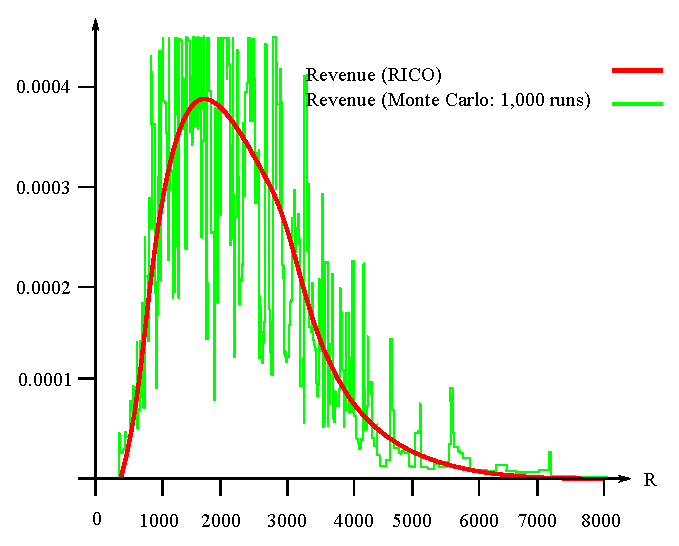
\includegraphics[width=2.33in, height=1.75in]{Images/ABC_1K}
\end{minipage}
\begin{minipage}[b]{0.5\linewidth}
\centering
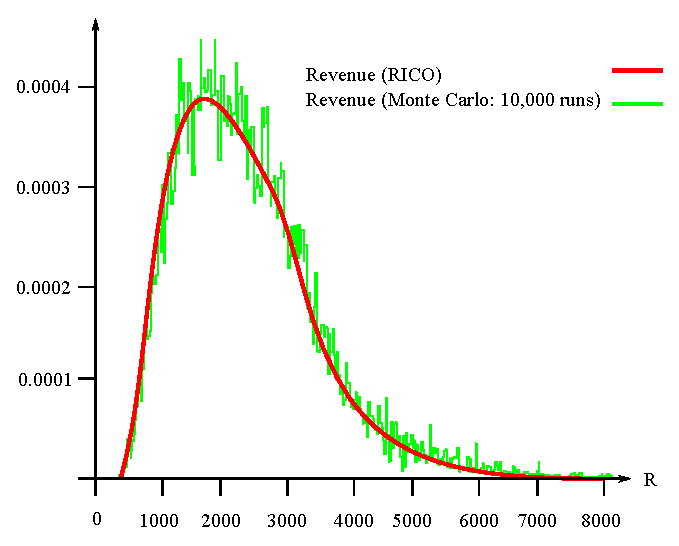
\includegraphics[width=2.33in, height=1.75in]{Images/ABC_10K}
\end{minipage}
\begin{minipage}[b]{0.5\linewidth}
\centering
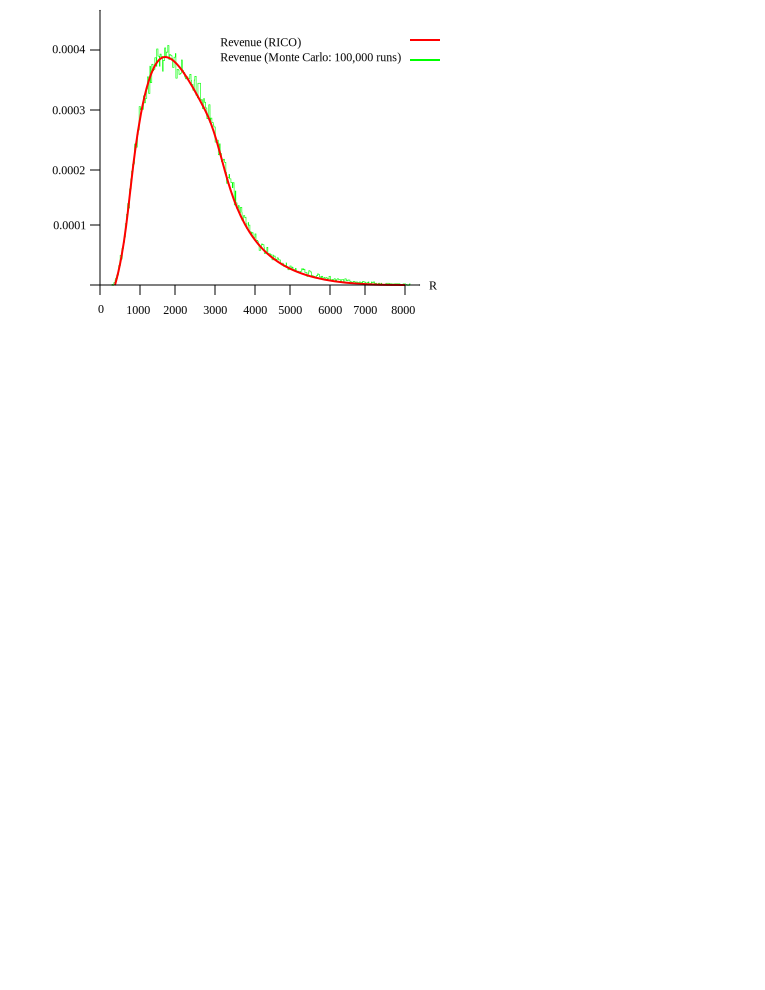
\includegraphics[width=2.33in, height=1.75in]{Images/ABC_100K}
\end{minipage}
\begin{minipage}[b]{0.5\linewidth}
\centering
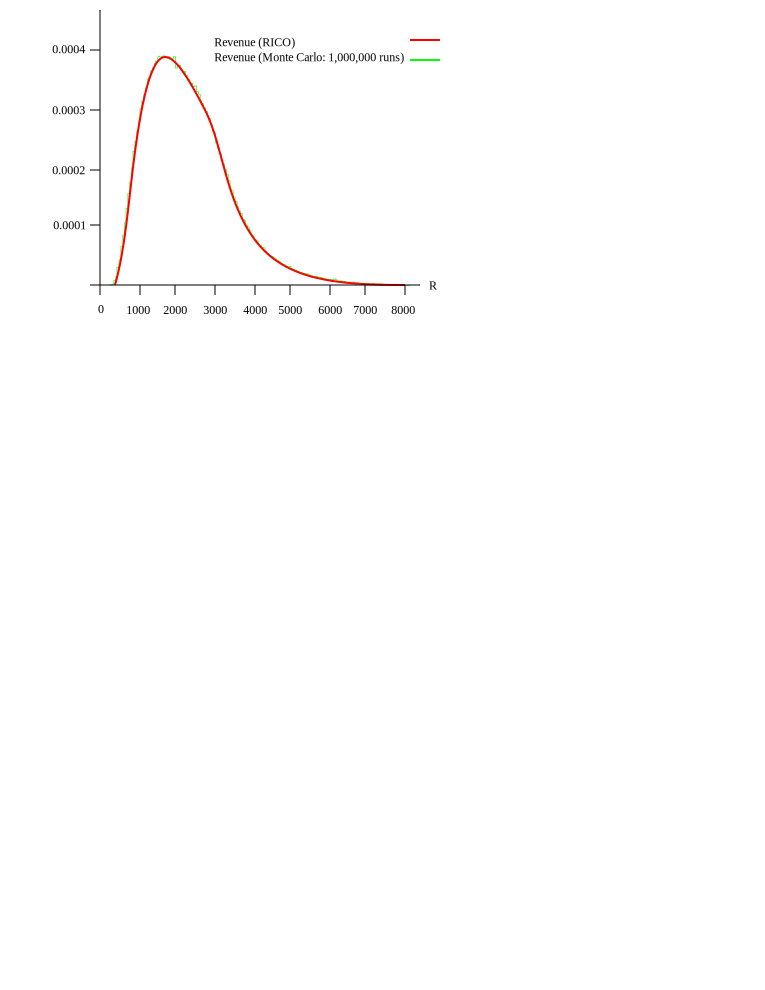
\includegraphics[width=2.33in, height=1.75in]{Images/ABC_1M}
\end{minipage}
  \caption[Random Revenue from Sales Combinations]
          {Random Revenue from Sales Combinations}
  \label{fig:ABC_4}
\end{figure}



Notable features of the optimized revenue in any panel of figure \ref{fig:ABC_4} is that no matter what happens with the projected demand there is a non-zero minimum revenue (about \$300), a strongly likelihood of earning about \$2200 and significant possibility of earning considerably more than the median \$2200.

Use the machinery developed above to convert the 3D price arrays to random variables. Since there is no optimization involved in computing prices there is no need to generate masks. Since some information is available about the range of prices to expect price partitions may be chosen directly. In this case each price is partitioned into regularly spaced intervals from 0 to \$150. The 3D probability arrays are projected onto the price partitions and the result for each price random variable is shown in figure \ref{fig:tcd_prices}. Notice that, by design, the price of chairs is has a median price of about \$45 and that of tables is about \$80 which corresponds with the sharp version of the tables and chairs example. 

\begin{figure}
  \centering
  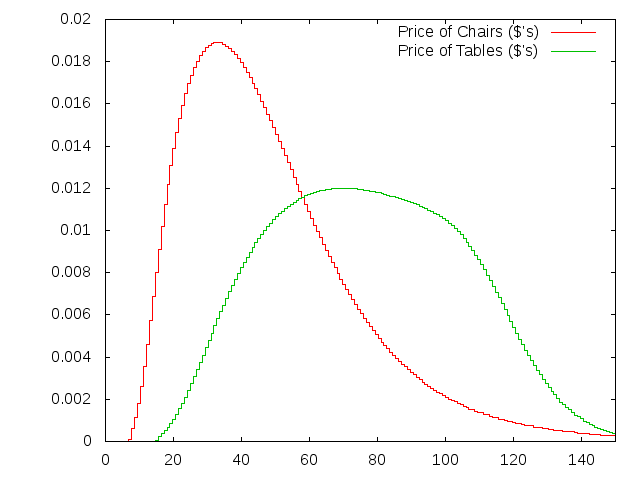
\includegraphics[width=120mm]{Images/tcd_prices}
  \caption[Random Variable Table and Chair Prices]
          {Random Variable Table and Chair Prices}
  \label{fig:tcd_prices}
\end{figure}

Notice that the price random variables are marginal probability distributions for a joint probability distribution are not computed. Since the price for tables and chairs are non-trivially correlated the joint distribution cannot be recovered from the marginal distributions alone as described in a standard statistics textbook such as \cite{bickel01}. 

\subsection{Finding the Joint Price Distribution from the Demand Inputs}

The reader will notice that the tables and chairs example with unknown prices is developed in preparation for the introduction of random inputs resulting in correlated prices. How to proceed with a joint distribution was described for the two prices, tables and chairs. Then the problem was solved without using, or even finding, the joint price distribution. Instead the 3D array was created to represent the three demand inputs. For this problem this technique provides directed and satisfactory results.

In this section the tables and chairs is revisited example with the same three demand input, but this time produce the joint price probability distribution. Since so much of this work is devoted to the study of correlated random variables it would be remiss not to include at least one example of same.

The problem with three 3D demand arrays, $DT$, $DC$ and  $DD$ is now revisted. The associated 3D probability array $DP$ is also available. Using the same formulas as before for finding the (correlated) prices of tables and chairs the two 3D price arrays $PT$ and $PC$ respectively follow. 

Each 3D price array may be projected onto a price partition and produced random variable representations of the two prices in figure \ref{fig:tcd_prices}. Choose the same price partitions as before, evenly space intervals from \$0 to \$150. This choice allows for comparable results with those obtained previously.

The two price partitions, for $PT$ and $PC$, describe a 2D partition of the $(Pc,Pt)$-space. If the number of points in each price partition is $Np$ then a 2D array of size $Np^2$ is created and initialized with zero values.

Notice that the two 3D price arrays $PT$ and $PC$ together describe a 3D lattice of pairs of prices at each vertex surrounding a uniform distribution of probability described by the 3D probability array $DP$. The 8 vertices of each probability block, each containing the two price values, are projected onto the two dimensional $(Pc, Pt)$-space. This the 2D analog of the 1D procedure for finding each marginal price random variable by projecting each price block for $PT$ or $PC$ onto the corresponding one dimensional price line. Figure \ref{fig:ptc_rectangle} shows an example of price block vertex projection. 

\begin{figure}
  \centering
  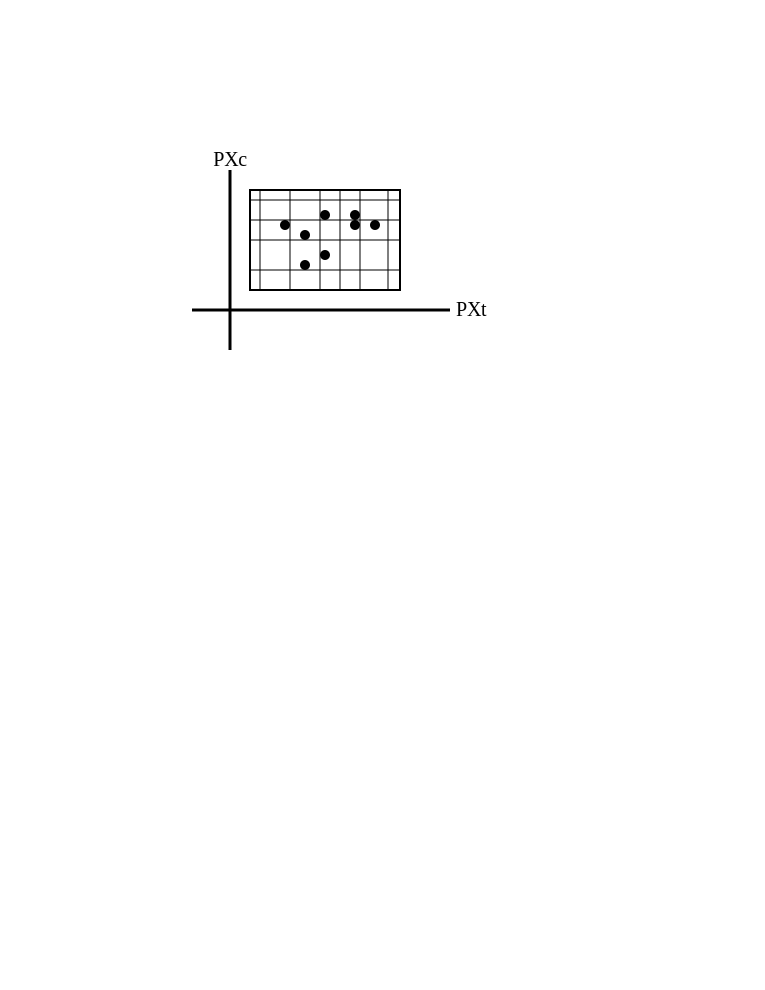
\includegraphics[width=3in]{Images/ptc_rectangle}
  \caption[Joint Price Partition with Block Vertex Projections]
          {Joint Price Partition with Block Vertex Projections}
  \label{fig:ptc_rectangle}
\end{figure}

Since the cluster of vertex projections in figure \ref{fig:ptc_rectangle} indicate the projection of the 3D price probability block onto the 2D joint price partition the block probability must be allocated accordingly. 

Assuming that the cluster of vertex projections represent the limits of the block projection the convex hull of these points may be found using an algorithm such as the Graham Scan as described in a textbook of computer algorithms such as Corman \cite{corman09}. Assume the block probability is distributed uniformly over the interior region of the convex hull and apportion it accordingly to the partition rectangles of the 2D price distribution, called $JP$. Figure \ref{fig:ptc_rectangle_convex} shows the convex hull of the projected vertices. The heavy outline of joint price rectangles shows the limits of affected rectangles. Let $p$ be the probability of the projected block and $a$ the area of the convexregion, then $h = p/a$ is the probability density. The portion of probability allocated to any given rectangle in the outlined region is $h$ times the area of the rectangle intersecting the convex region.

\begin{figure}
  \centering
  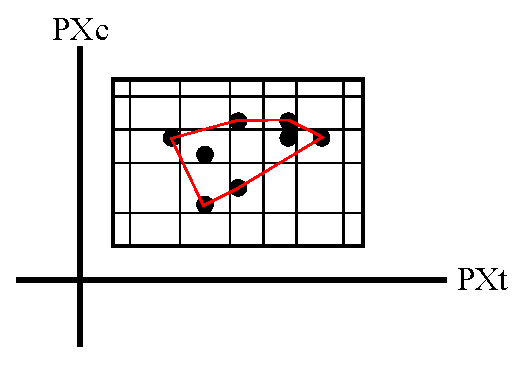
\includegraphics[width=3in]{Images/ptc_rectangle_convex}
  \caption[Joint Price Partition with Convex Block Projection]
          {Joint Price Partition with Convex Block Projection}
  \label{fig:ptc_rectangle_convex}
\end{figure}

The tables and chairs example has over 5 million blocks to project so a complex computation of multiple rectangle intersections with convex regions associated with each block is avoided for the prototype code. A simpler, though less accurate, approach is shown in figure \ref{fig:ptc_rectange_rectangle}. The heavy outline bounding box represents the $Pt$ and $Pc$ partition limits bounding the block vertex cluster. The shaded inner rectangle represents the rectangular limits of the cluster points. Calculate the probability density of the block probability as if distributed uniformly over the inner shaded rectangle and distribute this by area over each intersecting price rectangle. 

\begin{figure}
  \centering
  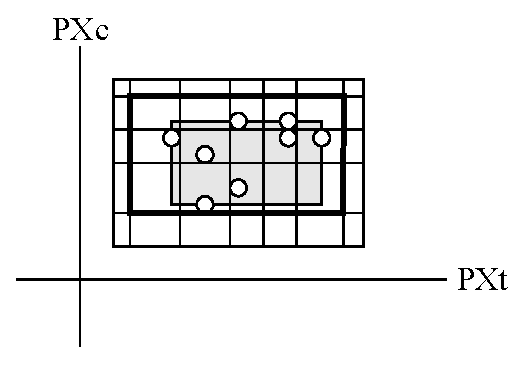
\includegraphics[width=3in]{Images/ptc_rectangle_rectangle}
  \caption[Joint Price Partition with Rectangular Block Projection]
          {Joint Price Partition with Rectangular Block Projection}
  \label{fig:ptc_rectange_rectangle}
\end{figure}

The results of the calculations of the prototype code for the joint probability distribution of the two correlated prices is shown in figure \ref{fig:Ptc}. Be aware that the origin is located in the upper-left corner of the graph. The $x$ and $y$ axis are prices of tables and chairs respectively and the vertical axis is probability density.
\begin{figure}
  \centering
  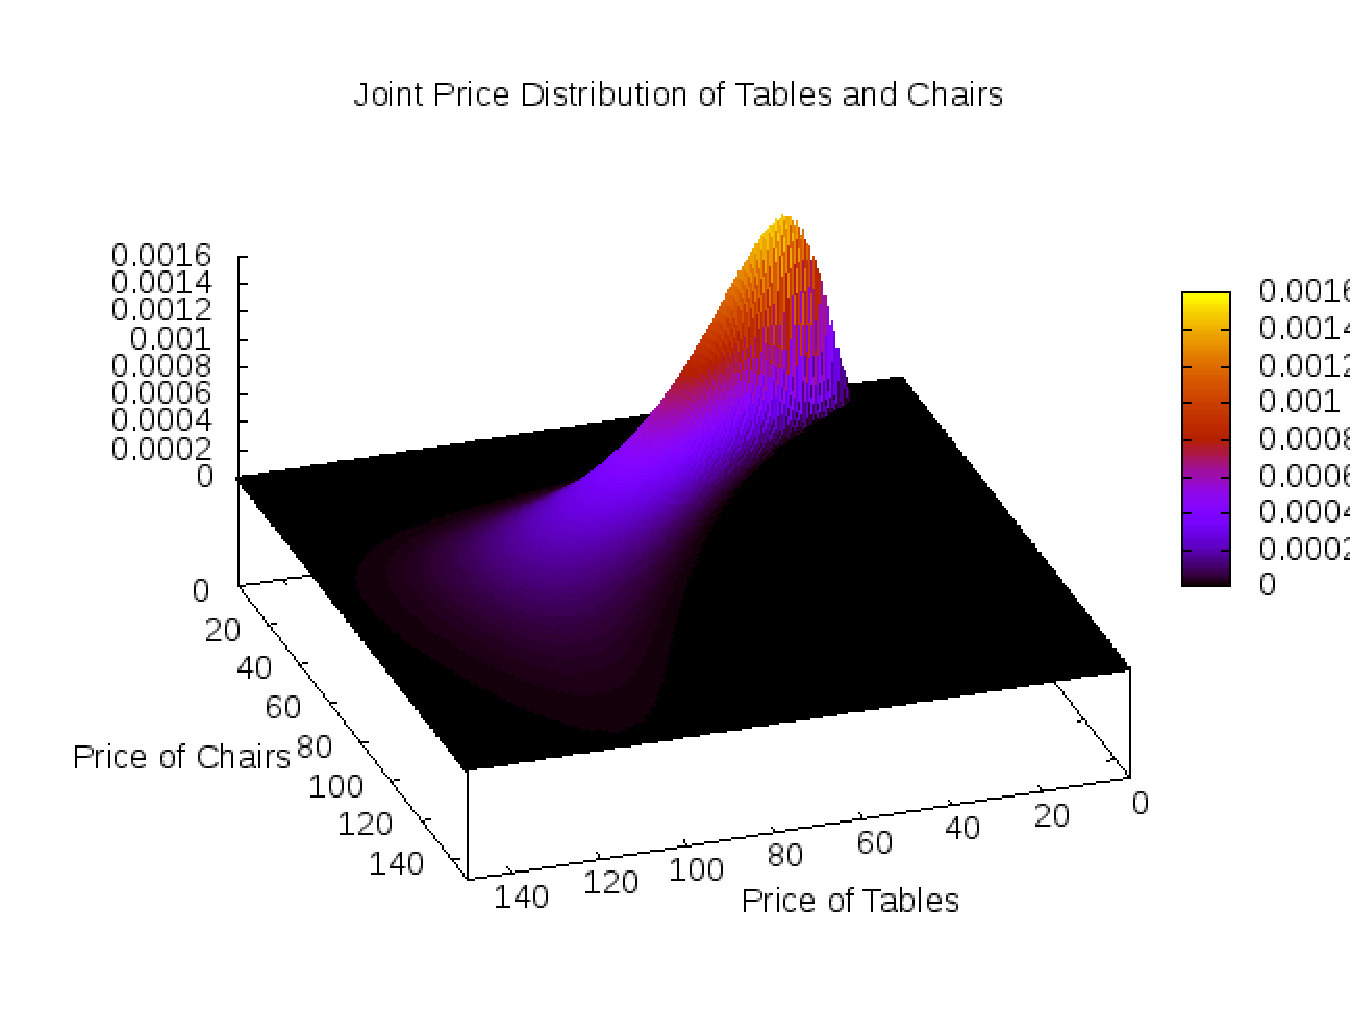
\includegraphics[width=120mm]{Images/Ptc.eps}
  \caption[Joint Probability Distribution of Table and Chair Prices]
          {Joint Probability Distribution of Table and Chair Prices}
  \label{fig:Ptc}
\end{figure}

An top view of the joint probability price distribution is shown figure \ref{fig:Ptc_flat}. Compare this figure to the original suggestion of the joint probability distribution of prices in figure \ref{fig:tc_joint_prices}. 

\begin{figure}
  \centering
  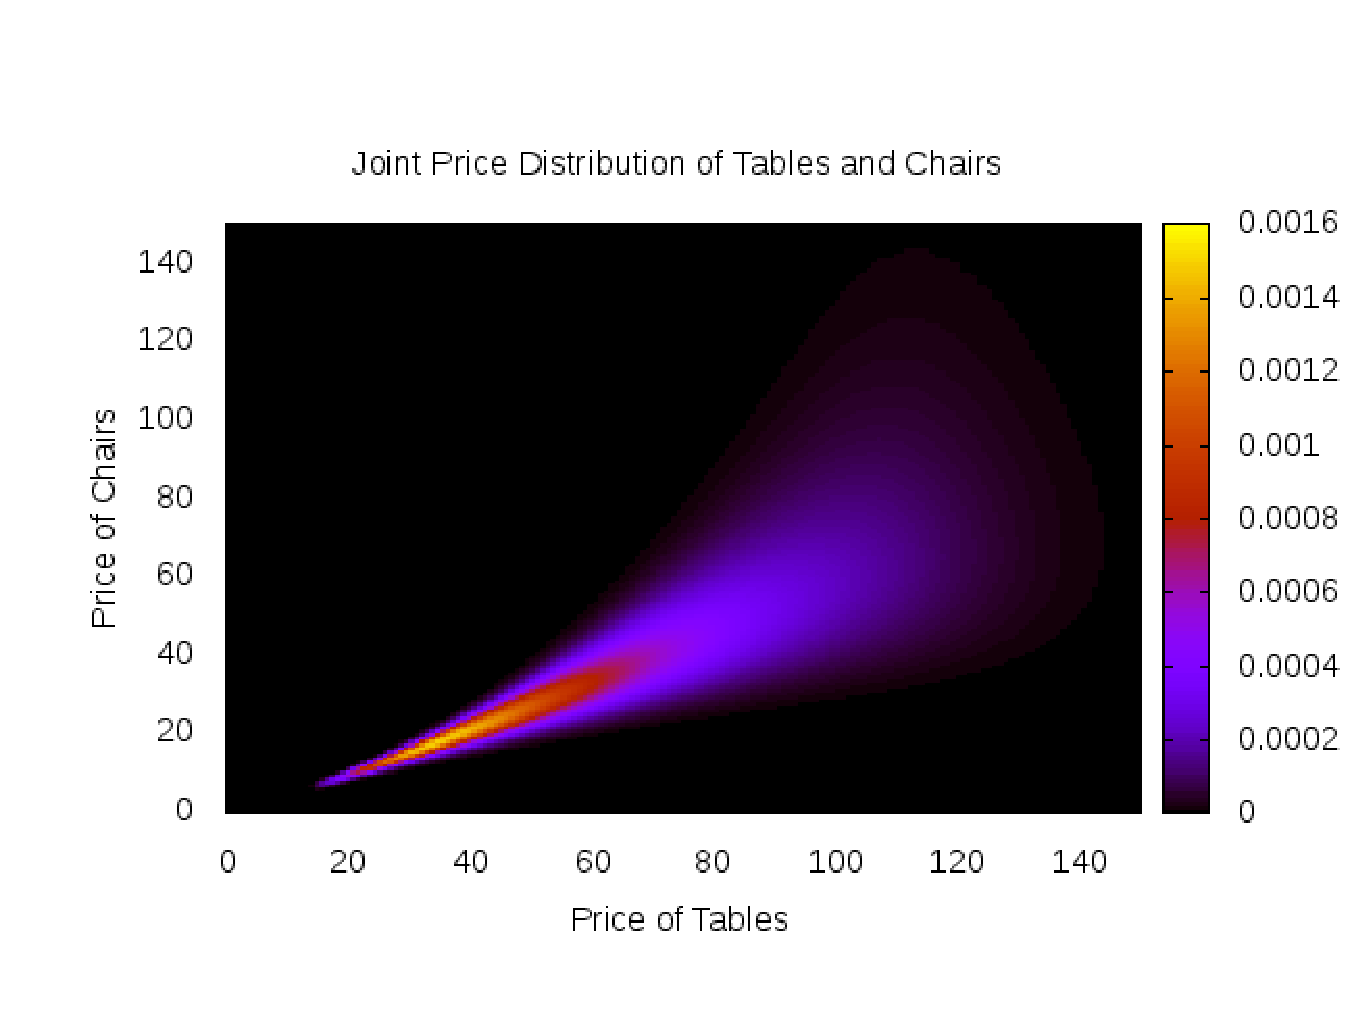
\includegraphics[width=120mm]{Images/Ptc_flat.eps}
  \caption[Joint Probability Distribution of Table and Chair Prices (Top View)]
          {Joint Probability Distribution of Table and Chair Prices (Top View)}
  \label{fig:Ptc_flat}
\end{figure}

It is interesting to note that the marginal random variable prices computed with the prototype code are identical to the random variable price computed previously and show in figure \ref{fig:tcd_prices}.

With the joint distribution of prices in hand the question of how to compute the probability of each branch in the simplex graph (see figure \ref{fig:tc_directed_graph}) is addressable. The probabilities of the branch conditional expressions are of particular interest,

\begin{align*}
p_t &< p_c\\
\frac{2}{3}p_t &< p_c\\
\frac{2}{3}p_t &< p_c < p_t\\
\frac{1}{4}p_t &< p_c\\
\frac{1}{4}p_t &< p_c < \frac{2}{3}p_t
\end{align*}

Proceeding as before, but starting with the jointly distributed prices and their partitions $P_t$ and $P_c$ 2D arrays $PT_2$ and $PT_2$ are created parallel to the 2D joint probability distribution array $JP$. Taking the last inequality above as an example each expression is devided by $p_t$ to find,

\begin{align*}
\frac{1}{4} < \frac{p_c}{p_t} < \frac{2}{3}
\end{align*}

In the prototype the 2D array expression $Qtc$ is formed as,

\begin{align*}
Qtc = \frac{PC_2}{PT_2}
\end{align*}

as the element-wise quotient of the two 2D price arrays. Notice that $Qtc$ together with the $JP$ form an improper form two-dimensional random variable, a non-standard usage of the expression. If a 1D partition is chosen for $Qtc$ the $\{Qtc, JP\}$ pair can be projected onto this partition and find a proper-form random variable, called $qtc$. This case is addressable by choosing the special partition,

\begin{align*}
Xqtc = (-\infty, 0, \frac{1}{4}, \frac{2}{3}, 1, \infty)
\end{align*}

The result is,

\begin{align*}
Pqtc = (0, 0.0001012, 0.7206, 0.2388, 0.03024, 0)
\end{align*}

Combining these into the random variable $Q$ for convenience as,

\begin{align*}
Q = \{Xqtc, Pqtc\}
\end{align*}

These probability values tell us probability of each simplex directed graph branch and therefore the probability of each result. For example, referring to figure \ref{fig:tc_directed_graph}, the probability of taking the first left directed edge under the condition that $p_t < p_c$ is  $\mathbb{P}(1 < Q) = 0.03024$. Similarly the probability of reaching result $B$ is $\mathbb{P}(\frac{1}{4} < Q < \frac{2}{3}) = 0.7206$.

\subsection{Tables and Chairs with Unknowns Prices and Resources}

Allowing prices and resources to be described by correlated random variables the impact on the example is to increase the number of branches from each simplex algorithm states and an increase in the number of states. The simplex tableau for unknown prices and resources is shown in table \ref{tab:pr0011}. 

\begin{table}
\centering
\begin{tabular}{| l | c c c c | c |}
\hline
0011    & $x_c$ & $x_t$ & $s_W$ & $s_L$ & $b$\\
\hline
$s_W$   & 5     & 20    & 1     & 0     & $b_W$\\
$s_L$   & 10    & 15    & 0     & 1     & $b_L$\\
\hline
Revenue & $p_c$    & $p_t$    & 0     & 0     &\\
\hline
\end{tabular}
  \caption[Tables and Chairs Simplex Tableau for Unknown Prices and Resources]
          {Tables and Chairs Simplex Tableau for Unknown Prices and Resources}
  \label{tab:pr0011}
\end{table}

The directed graph for the tables and chairs example with unknown prices and resources is shown in figure \ref{fig:tcpr_directed_graph}. Notice that there are only $\mathbb{C}(4,2) = 6$ possible node states in this example. Notice also that there are $5$ possible terminal states; manufacture of only tables or only chair limited by either wood resource or labor resource and also the mixed case.  

\begin{figure}
  \centering
  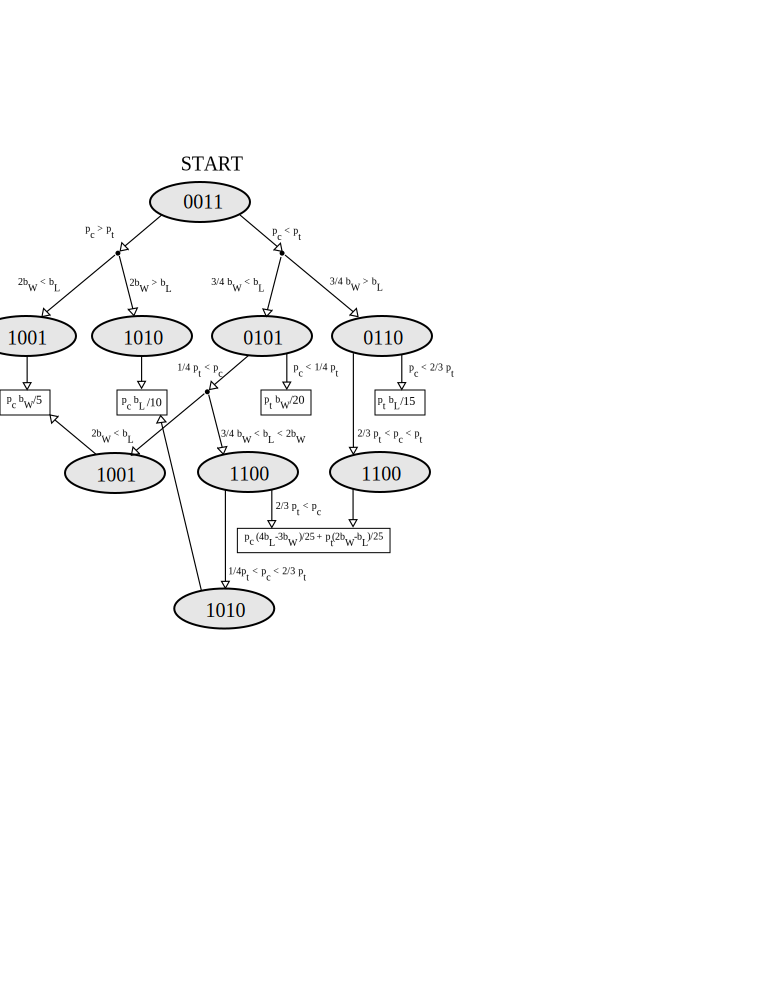
\includegraphics{Images/tcpr_directed_graph}
  \caption[Directed Graph for Tables and Chairs with Unknown Prices and Resources]
          {Directed Graph for Tables and Chairs with Unknown Prices and Resources}
  \label{fig:tcpr_directed_graph}
\end{figure}

While the conditions present when entering a state are significant, the tableau in each state is denumerable as. Refer to tables \ref{tab:pr1001}, \ref{tab:pr1010}, \ref{tab:pr0101}, \ref{tab:pr0110} and \ref{tab:pr1100}. 

\begin{table}
\centering
\begin{tabular}{| l | c c c c | c |}
\hline
1001    & $x_c$ & $x_t$ & $s_W$ & $s_L$ & $b$\\
\hline
$s_W$   & 1     & 4      & $\frac{1}{5}$   & 0     & $\frac{b_W}{5}$\\
$s_L$   & 0     & -25    & -2              & 1     & $b_L - 2b_W$\\
\hline
Revenue & $p_c$    & $p_t$    & 0     & 0     &\\
\hline
\end{tabular}
  \caption[Tableau for Unknown Prices and Resources, State 1001]
          {Tableau for Unknown Prices and Resources, State 1001}
  \label{tab:pr1001}
\end{table}

\begin{table}
\centering
\begin{tabular}{| l | c c c c | c |}
\hline
1010    & $x_c$ & $x_t$ & $s_W$ & $s_L$ & $b$\\
\hline
$s_W$   & 1     & $\frac{3}{2}$  & 0   & $\frac{1}{10}$  & $\frac{b_L}{10}$\\
$s_L$   & 0     & -25            & 1   & -$\frac{1}{2}$  & $b_W - \frac{b_L}{2}$\\
\hline
Revenue & $p_c$    & $p_t$    & 0     & 0     &\\
\hline
\end{tabular}
  \caption[Tableau for Unknown Prices and Resources, State 1010]
          {Tableau for Unknown Prices and Resources, State 1010}
  \label{tab:pr1010}
\end{table}

\begin{table}
\centering
\begin{tabular}{| l | c c c c | c |}
\hline
0101    & $x_c$ & $x_t$ & $s_W$ & $s_L$ & $b$\\
\hline
$s_W$   & $\frac{1}{4}$   & 1  & $\frac{1}{20}$   & 0  & $\frac{b_W}{20}$\\
$s_L$   & $\frac{25}{4}$  & 0  & -$\frac{3}{4}$   & 1  & $b_L - \frac{3}{4}b_W$\\
\hline
Revenue & $p_c$    & $p_t$    & 0     & 0     &\\
\hline
\end{tabular}
  \caption[Tableau for Unknown Prices and Resources, State 0101]
          {Tableau for Unknown Prices and Resources, State 0101}
  \label{tab:pr0101}
\end{table}

\begin{table}
\centering
\begin{tabular}{| l | c c c c | c |}
\hline
0110    & $x_c$ & $x_t$ & $s_W$ & $s_L$ & $b$\\
\hline
$s_W$   & $\frac{2}{3}$    & 1  & 0  & $\frac{2}{30}$  & $\frac{b_L}{15}$\\
$s_L$   & -$\frac{25}{3}$  & 0  & 1  & -$\frac{4}{3}$  & $b_W - \frac{4}{3}b_L$\\
\hline
Revenue & $p_c$    & $p_t$    & 0     & 0     &\\
\hline
\end{tabular}
  \caption[Tableau for Unknown Prices and Resources, State 0110]
          {Tableau for Unknown Prices and Resources, State 0110}
  \label{tab:pr0110}
\end{table}

\begin{table}
\centering
\begin{tabular}{| l | c c c c | c |}
\hline
1100    & $x_c$ & $x_t$ & $s_W$ & $s_L$ & $b$\\
\hline
$s_W$   & 1  & 0  & -$\frac{3}{25}$  & $\frac{4}{25}$  & $\frac{4b_L-3b_W}{25}$\\
$s_L$   & 0  & 1  & $\frac{2}{25}$  & -$\frac{1}{25}$  & $\frac{2b_W-b_L}{25}$\\
\hline
Revenue & $p_c$    & $p_t$    & 0     & 0     &\\
\hline
\end{tabular}
  \caption[Tableau for Unknown Prices and Resources, State 1100]
          {Tableau for Unknown Prices and Resources, State 1100}
  \label{tab:pr1100}
\end{table}

Starting in state $0011$ and following the simplex two-phase decision and first compare the two prices $p_c$ and $p_t$. Assuming for clarity, as before, that since it is intended to replace $p_c$ and $p_t$ with continuous random variables the probability of equality is zero. In practice the possibility of equality must be checked. The initial comparisons are,

\begin{align*}
argmax(p_c, p_t)\\
argmin(\frac{b_W}{5}, \frac{b_L}{10}  | > 0 \text{ and } p_c > p_t)\\
argmin(\frac{b_W}{20}, \frac{b_L}{15} | > 0 \text{ and } p_c < p_t)
\end{align*}

where the $> 0$ condition refers to the requirement that each operand be positive else it is disqualified from the comparison.

%4/21/2011 p.2

In many cases the first or second phase of the simplex algorithm decision is disqualified since it is either non-positive or contradicts a previous assumption. 

Since simplex states may be re-entered a computer algorithm can take advantage of this possibility and cache, rather than recompute, certain elements such as the simplex tableau. Notice the comparison of linear combinations of either price or resource variables with zero, at each decision potin, in the sense that the expression $a < b$ can be rewritten as $0 < b - a$. Recall from the previous version of the tables and chairs example that each conditional statement results in a filter on the input space so that the simplex algorithm may be viewed as a filtration process. The task of the RICO modeling environment is to determine what portion of the input space passes through each facet of the simplex filtration process to a terminal node and with what probability.

\section{Beyond the Tables and Chairs Example}

In the tables and chairs example correlated random inputs for prices were chosen and it was argued that correlated random inputs could have been chosen for resources instead. Notice in the simplex algorithm the transition decision from one state to the other involves computing the maximum positive revenue impact in the case of prices and then the minimum positive resource impact. These two choices correspond to the two facets of a table pivot as explained above. 

It remains to be investigated what happens to this example when some or all of the values of $A$ are unknown. In this example the significance of unknown $A$ values is that the manufacturer is unsure how many resources are consumed by each product.

As explained by Bellman \cite{bellman03}, the number of solution states, not to mention the number of internal simplex algorithm states, becomes computationally intractable even for modest problems. Notice that if the problem has 100 variables and 100 constraints then the number of simplex states is at least $\mathbb{Ch}(200,100) = 9.05\times10^{58}$. The reference implementation of the AB32 model has many hundreds of variables and several thousand constraint equations. 

A way to proceed is for the RICO modeling environment to partially explore the simplex directed graph. The transition from one state to the next using the simplex algorithm involves finding the maximum of a set of linear combinations of prices, in the context of the tables and chairs example, followed by finding the minimum of a set of linear combinations of resource limits assuming the $A$ values are fixed. Each \emph{choice element} is a linear combination of random variables which are themselves random variables. Assuming that there are three choice elements denoted $X$, $Y$ and $Z$ then the decision,

\begin{align*}
argmax\{X, Y, Z\}
\end{align*}

results in three probability values,

\begin{align*}
\mathbb{P}(X < \{Y, Z\})\\
\mathbb{P}(Y < \{X,Z\})\\
\mathbb{P}(Z < \{X,Y\})
\end{align*}

In this case the simplex algorithm state has three initial branches corresponding to the first decision of the pivot element. These probabilities may be computed explicitly and rather than create a directed graph with all choices listed as done above with the tables and chairs directed graph, choose only the most highest probability transition. In this manner a terminal node is reached as in the sharp version of the simplex algorithm. 

Since it's possible to assign probability values to each transition edge in the directed graph a choice algorithm may be applied to explore other paths based on their likelihood of occurrence. As long as the directed graph remains at least partly unexplored, it is suspected that this is the case in general, then the random variable results will not have \emph{full   probability}, that is, their probability values will sum to less than one. The proximity of the probability sum of a random variable result to unity can be used as a criterion for algorithm termination. That is, if the random variable result is deemed near enough to completion the algorithm can terminate its exploration of the simplex directed graph.


\chapter{Black Scholes Construction}
\section{Black Scholes Construction}

Consider a financial security such as a stock $S$ with current market price $S_0$. At some future time $T$ let the price of $S$ be represented by a random variable $S_T$ whose probability distribution is indicated in figure \ref{fig:S_T}. Here, no presumption is yet made about the kind of distribution for $S_T$. 

\begin{figure}
  \centering
  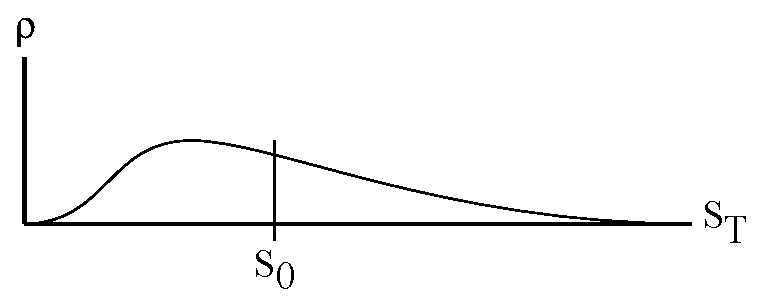
\includegraphics[width=2.5in]{Images/S_T.eps}
  \caption[Distribution of Stock Prices at time T]
          {Distribution of $S_T$}
  \label{fig:S_T}
\end{figure}

Following Dineen \cite{dineen00} suppose now that $S_T$ satisfies the so-called \emph{no-arbitrage requirement} $S_0 = \mathbb{E}[S_T]$. Suppose an investor, Ivan, holds one unit of stock $S$ as the sole content of his portfolio of assets. Initially his wealth $W$ is then just,

\begin{align*}
W_0 = S_0
\end{align*}

and at time $T$ his wealth is expressed as,

\begin{align*}
W_T = S_T
\end{align*}

Expressing Ivans future wealth in terms of his current wealth and a continuously compounding growth rate $r$ one writes

\begin{align*}
W_T = W_0 e^{r_T}
\end{align*}

where

\begin{align*}
r_T = log(\frac{S_T}{S_0}).
\end{align*}

Referring to $\hat{S_T} = S_T / S_0$ as the \emph{normalized} stock price rescale the probability distribution $S_T$ to $\hat{S_T}$ so that the mean of $\hat{S_T}$ is one as depicted in figure \ref{fig:S_T_hat}.

\begin{figure}
  \centering
  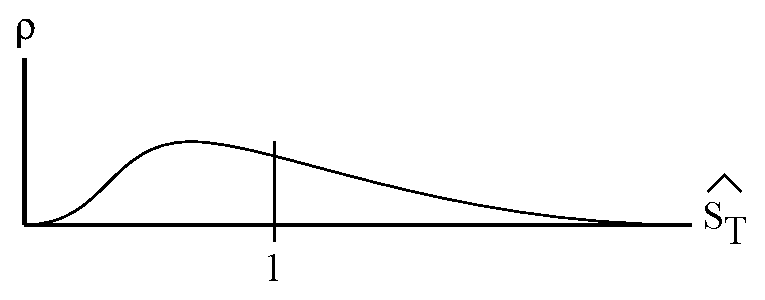
\includegraphics[width=2.5in]{Images/S_T_hat.eps}
  \caption[Distribution of Normalized Stock Price at time T]
          {Distribution of $\hat{S_T}$}
  \label{fig:S_T_hat}
\end{figure}

Since $r_T$ is the log of $\hat{S_T}$, its mean is zero as illustrated in figure \ref{fig:r_T}. Notice that if $\hat{S_T}$ is represented by a LogNormal random variable then $r_T$ is represented by a Normal random variable with zero mean.

\begin{figure}
  \centering
  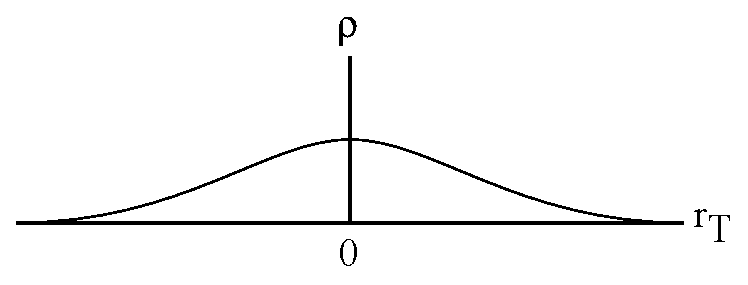
\includegraphics[width=2.5in]{Images/r_T.eps}
  \caption[Distribution of Return Rate at time T]
          {Distribution of $r_T$}
  \label{fig:r_T}
\end{figure}

If instead of holding a unit of stock $S$, the investor Ivan holds a European-style call option $C$ based on stock $S$ with strike price $K$ exercisable at time $T$. The value of $C$ at time $T$ is given by

\begin{align*}
C_T = [S_T - K]^+
\end{align*}

similarly, the related put-option $P$ with the same parameters as $S$ has value $P_T$ at time $T$ with

\begin{align*}
P_T = [S_T - K]^-
\end{align*}

It is helpful to notice that $C_T, P_T \ge 0$. For ease of calculation, the assumption is made that upon maturity all options are settled in cash and that there is no requirement that the \emph{underlying} stock be transferred between parties. A further assumption made here is that all cash values are stated in current (t = 0) dollars. Please note that this runs counter to the not uncommon practice in financial texts, e.g. \cite{dineen00} to include the effect of time-value-of-money in calculations. While the current dollars assumption is equivalent to zero interest rate, the understanding is that all cash may be restated in any chosen year denomination.

To find the probability distribution over the mature value $C_T$ of the call option $C$ at time $T$ with the underlying stock $S$ and strike price $K$, a sequence of transformations of $S_T$ are necessary. The first transformation is to subtract the strike price $K$ from the distribution $S_T$. The resulting distribution is illustrated in figure \ref{fig:S_T_minus_K}. The key feature is represented by the shaded region in figure \ref{fig:S_T_minus_K} is the probability $q$, such that $q = Pr\{S_T - K \le 0\}$. 

\begin{figure}
  \centering
  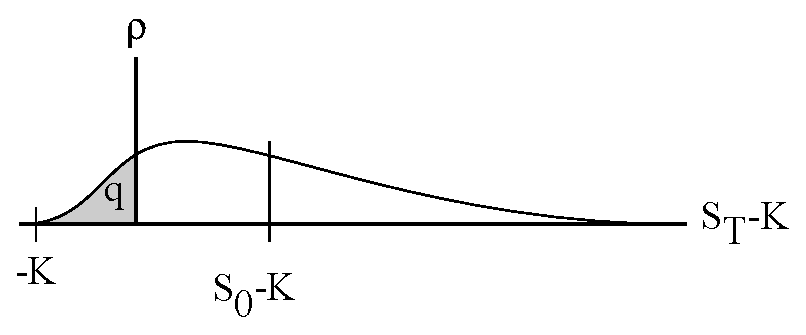
\includegraphics[width=2.5in]{Images/S_T_minus_K.eps}
  \caption[Distribution of $S_T$ Minus Strike Price $K$]
          {Distribution of $S_T - K$}
  \label{fig:S_T_minus_K}
\end{figure}

The second transformation, the probability distribution of $[S_T - K]^+$ is illustrated in figure \ref{fig:S_T_minus_K_plus}. Notice that the probability $q$ is now concentrated discretely at zero and represented by a vertical arrow labeled $q$. Since the remaining portion of the distribution is continuously distributed, the vertical axis still represents probability density. Notice further that the mean $\mu_{C_T}$ of this mixed, continuous/discrete probability distribution, is indicated at some positive location in figures. Notice that as $C_T = [S_T - K]^+$,

\begin{align*}
\mu_{C_T} = \mathbb{E}[[S_T - K]^+] = \mathbb{E}[C_T]
\end{align*}

The significance of $\mu_{C_T}$ in figure \ref{fig:S_T_minus_K_plus} is that this price, based on the no-arbitrage principle, an investor can expect to pay today $(t = 0)$ for a call of this type when $S_T$ represents the commonly accepted probability distribution of the value of stock $S$ at time $T$. That is,

\begin{align*}
C_0 = \mu_{C_T} = \mathbb{E}[C_T]
\end{align*}

\begin{figure}
  \centering
  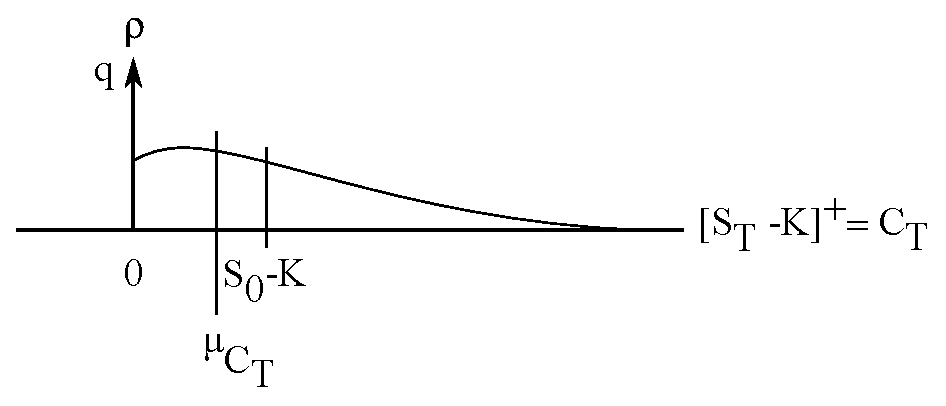
\includegraphics[width=2.5in]{Images/S_T_minus_K_plus.eps}
  \caption[Distribution of Positive Portion of $S_T$ Minus Strike Price $K$]
          {Distribution of $[S_T - K]^+$}
  \label{fig:S_T_minus_K_plus}
\end{figure}

Normalizing the distribution of the mature call option with respect to the initial value of the underlying $S_0$ gives the distribution for $\hat{C_T}$, the normalized call option price, illustrated in figure \ref{fig:C_T_hat}.

\begin{figure}
  \centering
  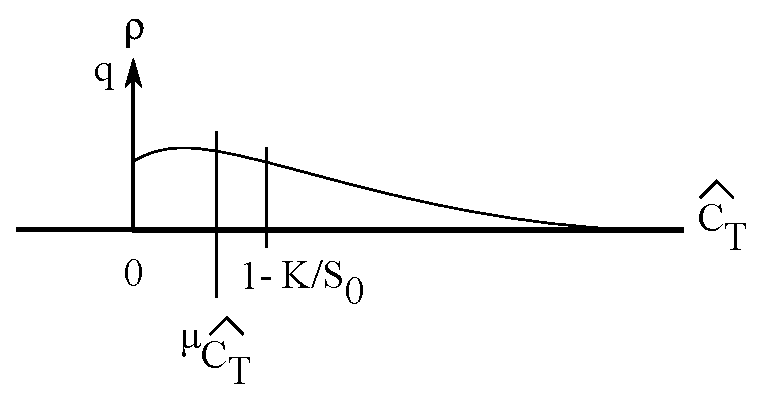
\includegraphics[width=2.5in]{Images/C_T_hat.eps}
  \caption[Distribution of Normalized Mature Call]
          {Distribution of $\hat{C_T}$}
  \label{fig:C_T_hat}
\end{figure}

Using the same strike price $K$ and underlying stock $S$, a put option value at maturity is illustrated in figure \ref{fig:S_T_minus_K_minus} where value at maturity of the put option is,

\begin{align*}
P_T = \mathbb{E}[[S_T - K]^-]
\end{align*}

and the no-arbitrage price of the put is,

\begin{align*}
P_0 = \mu_{P_T}
\end{align*}

Note that the probability concentrated at zero here is $1-q = Pr\{S_T - K < 0\}$.

\begin{figure}
  \centering
  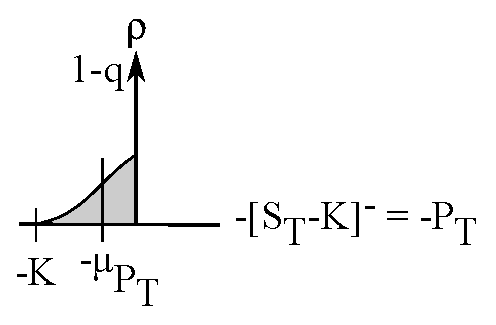
\includegraphics{Images/S_T_minus_K_minus.eps}
  \caption[Distribution of Negative Portion of $S_T$ Minus Strike Price $K$]
          {Distribution of $-[S_T - K]^-$}
  \label{fig:S_T_minus_K_minus}
\end{figure}

The \emph{put-call parity formula},

\begin{align*}
\mathbb{E}[C_T] - \mathbb{E}[P_T] = S_0 - K
\end{align*}

is now obtained easily using the notation stated above, noting that

\begin{align*}
\mathbb{E}[C_T] - \mathbb{E}[P_T] &= S_0 - K\\
\mathbb{E}[C_T - P_T] &= S_0 - K\\
\mathbb{E}[[S_T - K]^+ - [S_T - K]^-] &= S_0 - K\\
\mathbb{E}[S_T - K] &= S_0 - K\\
\mathbb{E}[S_T] - K &= S_0 - K\\
S_0 - K &= S_0 - K\\
\end{align*}

as in Dineen \cite{dineen00}, with the exception that Dineen \cite{dineen00} denotes as $C_T$ the expected value of the probability distribution denoted $C_T$ in this paper and similarly for $P_T$. 

There is a geometric interpretation of Put-Call Parity. This can be seen in the perspective figure \ref{fig:CP_addition}, where the probability density axis is perpendicular to the $C_T \times (−P_T)$-space. Put–Call Parity is realized in that figure as the elementary projection of the joint $C_T \times (−PT)$-space to the diagonal $C_T + (−P_T)$-space. The analogous algebraic calculation procedure is detailed in the appendix.

\begin{figure}
  \centering
  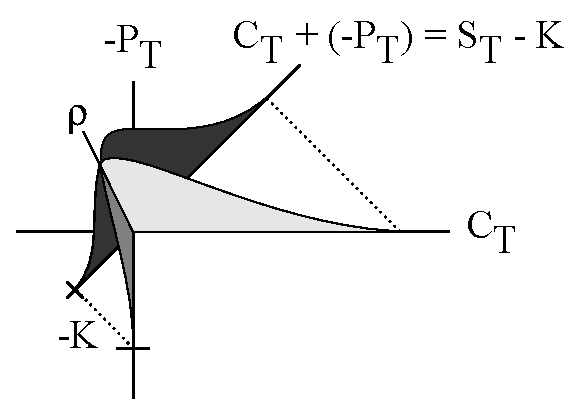
\includegraphics[width=3in]{Images/CP_addition.eps}
  \caption[Distribution of Put-Call Parity in Perspective]
          {Distribution of $C_T - P_T = S_T - K$ in Perspective}
  \label{fig:CP_addition}
\end{figure}

%%%%%%%%%%%%%%%%%%%%%%%%%%%%%%%%%%%%%%%%%%%%%%%%%%%%%%%%%%%%%%%%%%%%%%%%%%%%%%%%%%%%%%%%%%%%%%%

\subsection{Geometric Black-Scholes Pricing}

Suppose now that a random variable $X$ has probability density function $\rho(x)$ and is ``well behaved'' enough to have mean $M = \mathbb{E}[X] < \infty$. Suppose further we have a partition point $K$ as shown in figure \ref{fig:S_T_K_generic} and let $q = Pr\{X < K\}$ and so $1 - q = Pr\{X \ge K\}$.

\begin{figure}
  \centering
  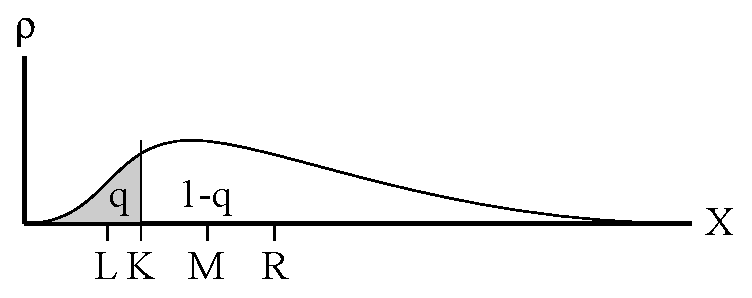
\includegraphics[width=2.5in]{Images/S_T_K.eps}
  \caption[Probability Distribution Partitioned at $K$]
          {Probability Distribution Partitioned at $K$}
  \label{fig:S_T_K_generic}
\end{figure}

Form two new \emph{truncated} random variables from the left and right sections of the $K$-partitioned random variable $X$ with probability densities,

\begin{align*}
X_L \sim \rho_L(x) &= \frac{\rho(x) \mathbf{1}_{X < K}}{q}\\
X_R \sim \rho_R(x) &= \frac{\rho(x) \mathbf{1}_{X \ge K}}{1-q}
\end{align*}

\begin{figure}
  \centering
  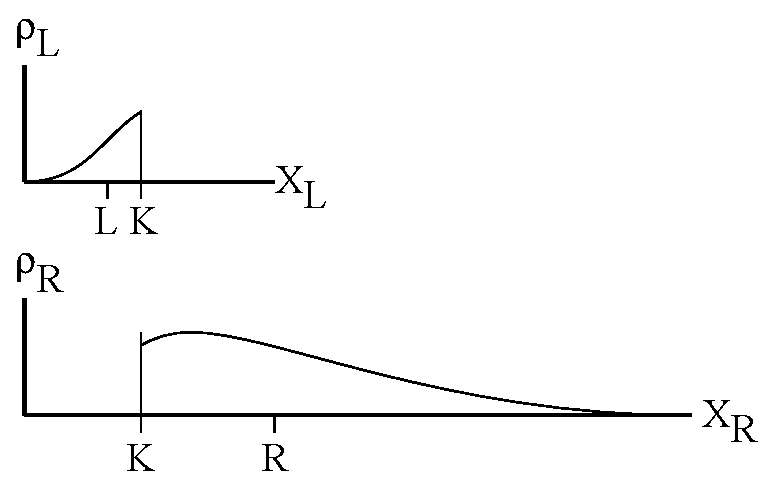
\includegraphics{Images/XL_XR.eps}
  \caption[Left- and Right-Truncated Random Variables]
          {Left- and Right-Truncated Random Variables}
  \label{fig:XL_XR}
\end{figure}

as depicted in figure \ref{fig:XL_XR} where the $L$ and $R$ are expected values of $X_L$ and $X_R$. Notice that the affine combination of $L$ and $R$ via $q$, illustrated in figure \ref{fig:XL_XR_M}, yields the original mean $M$,

\begin{align*}
M = q * L + (1-q) * R
\end{align*}

\begin{figure}
  \centering
  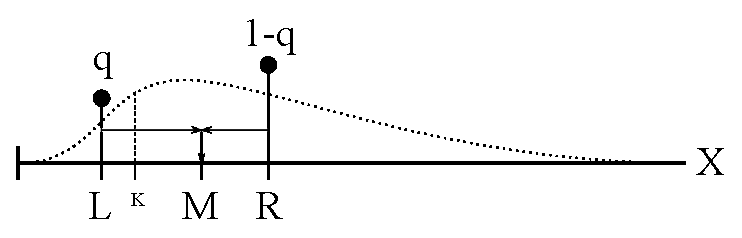
\includegraphics{Images/XL_XR_M.eps}
  \caption[Mean Relationship Between Bifurcated Sections]
          {Mean Relationship Between Bifurcated Sections}
  \label{fig:XL_XR_M}
\end{figure}

Toward Geometric Black-Scholes pricing define new random variables $Y = K + [X-K]^+$ and $Z$, a discrete random variable such that $Pr\{Z = K\} = 1$ with discrete density $\rho_Z = \mathbf{\delta}_{z = K}$. Then the density $\rho_Y$ of $Y$ is

\begin{align*}
\rho_Y(y) = q * \rho_z(y) + (1-q) * \rho_R(y)
\end{align*}

and depicted in figure \ref{fig:Z_XR_K}. Note in particular that $Y$ is a \emph{mixed} discrete and continuous random variable.

\begin{figure}
  \centering
  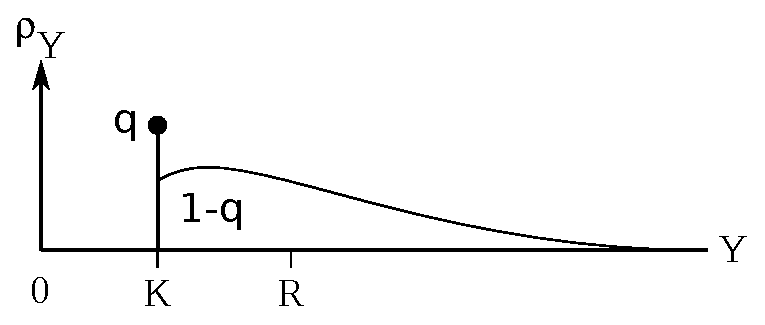
\includegraphics[width=2in]{Images/Z_XR_K.eps}
  \caption[Positive Density]
          {Positive Density}
  \label{fig:Z_XR_K}
\end{figure}

To compute the mean of $Y$, the $X_R$ portion of $Y$ may be replaced with a discrete density $(1-q)$ at the mean $R$ of $X_R$, as illustrated in figure \ref{fig:Z_XR_K_discrete}. The mean $M_Y$ of $Y$ is then the affine combination

\begin{align*}
M_Y = \mathbb{E}[Y] = q * K + (1-q) * R
\end{align*}

\begin{figure}
  \centering
  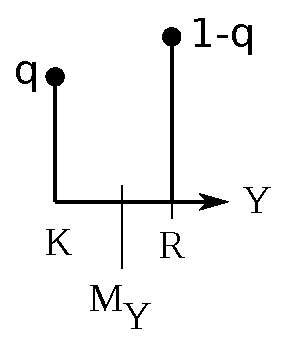
\includegraphics[width=0.75in]{Images/Z_XR_K_discrete.eps}
  \caption[Geometric Black-Scholes Pricing]
          {Geometric Black-Scholes Pricing}
  \label{fig:Z_XR_K_discrete}
\end{figure}

Finally Geometric Black-Scholes pricing requires computing the mean of $[X-K]^+$ for some random variable $X$ such that $\mathbb{E}[X] < \infty$ and constant $K$. Using the notation developed in this section the result is expressed immediately as

\begin{align*}
\mathbb{E}[[X-K]^+] &= \mathbb{E}[Y] - K
\end{align*}

and more conveniently as,

\begin{align*}
\mathbb{E}[[X-K]^+] + K &= q * K + (1-q) * R
\end{align*}

As an illustrative example the traditional Black-Scholes formula is recovered by letting $X = S_T$ be a LogNormally distributed random variable representing the stock price of the underlying asset at some future time $T$. To use Geometric Black-Scholes to price a European-style call option with maturity time $T$ and strike price $K$ let $C_T = [X-K]^+$ and find the current price of the call option as $C_0 = \mathbb{E}[C_T]$. Following the steps above symbolically first identify the probability density of $S_T$,

\begin{align*}
\rho(x) = \frac{1}{x \sqrt{2 \pi} \sigma} e^{-\frac{1}{2}(\frac{ln(x) - \mu}{\sigma})^2}
\end{align*}

Following Dineen \cite{dineen00}, the current price $S_0$ is the mean of $S_T$,

\begin{align*}
S_0 = \mathbb{E}[S_T] = e^{\mu + \frac{\sigma^2}{2}}.
\end{align*}

Since $S_0$ is a known quantity it may be used to solve for the unknown LogNormal parameter $\mu$,

\begin{align*}
\mu = ln(S_0) - \frac{\sigma^2}{2}
\end{align*}

and the parameter $\sigma$, according to standard interpretations, e.g. Dineen \cite{dineen00}, represents the asset volatility and must be given. The option price $C_0$ is expressed by the formula derived above as

\begin{align*}
C_0 + K &= q * K + (1-q) * R\\
C_0 &= (1-q) * R - (1-q) * K
\end{align*}

Finding the mean $R$ of the right-truncated LogNormal and its associated probability $(1-q)$,

\begin{align*}
R &= \frac{1}{1-q}\frac{1}{\sqrt{2 \pi} \sigma} \int_K^\infty e^{-\frac{1}{2}(\frac{ln(x) - \mu}{\sigma})^2} \; dx\\
&= \frac{1}{1-q} e^{\mu + \sigma^2 / 2} \Phi\left(\frac{-ln(K) + \mu + \sigma^2}{\sigma}\right)\\
&= \frac{1}{1-q} S_0 \Phi\left(\frac{ln(S_0/K) + \sigma^2 / 2}{\sigma}\right)
\end{align*}

and

\begin{align*}
1-q &= \Phi\left(-\frac{ln(K)-\mu}{\sigma}\right)\\
    &= \Phi\left(\frac{ln(S_0 / K) - \sigma^2 / 2}{\sigma}\right)
\end{align*}

where

\begin{align*}
\Phi(z) &= Pr(Z <= z) \; \text{ for } Z \sim Normal(\mu, \sigma^2)
\end{align*}

the traditional Black-Scholes formula follows immediately,

\begin{align*}
C_0 &= S_0 \Phi\left(\frac{ln(S_0 / K) + \sigma^2 / 2}{\sigma}\right) - K \Phi \left(\frac{ln(S_0 / K) - \sigma^2 / 2}{\sigma}\right)
\end{align*}

\subsection{Portfolio Construction}

Given a stock $S$ represented at time $t=0$ by value $S_0$ and at $t=T$ by random variable $S_T$ and a European call option $C$ based on $S$ with strike price $K$ at time $T$ the domain of the joint probability distribution of $S$ and $C$ is shown in figure \ref{fig:SC}. The point $(S_0, C_0)$ corresponds to the joint initial price of the stock and call. The broken line is the familiar curve for a call option graph. Perpendicular to the $SC-plane$ is the joint probability density of $S$ and $C$ at time $T$. The probability density is zero at points away from the broken line.

\begin{figure}
  \centering
  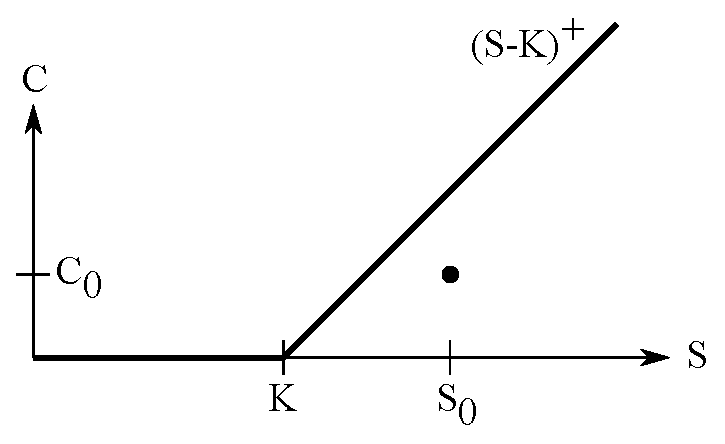
\includegraphics[width=3in]{Images/SC.eps}
  \caption[Stock-Call Space]
          {Stock-Call Space}
  \label{fig:SC}
\end{figure}

Since the $SC$-space represents the price per unit of each financial security there is a dual space where each point represents the number of units held in a hypothetical portfolio. This dual space is referred to here as the portfolio space. Given a portfolio vector $\pi$ and a point $w$ in $SC$ the dollar value of $pi$ at $w$ is $\pi^T\;w$. Recall that the projection matrix of $SC$ onto a vector $v$ in $SC$ is given by,

\begin{align*}
\Pi = \frac{v\;v^T}{v^T\;v}
\end{align*}

Notice that given portfolio $\pi = (\pi_s, \pi_c)$ the random variable $Z_T = \pi_s * S_T + \pi_c * C_T$ appears graphically as a hyperplane in $SC$-space. Notice in particular that if the projection vector in $SC$-space is $\pi$ itself then the projection matrix becomes,

\begin{align*}
\Pi = \frac{\pi\;\pi^T}{\pi^T\;\pi}
\end{align*}

and more to the point the portfolio value $V$ given $x \in SC$-space is,

\begin{align*}
V &= \pi^T\;x\\
  &= \pi^T \frac{\pi\;\pi^T}{\pi^T\;\pi} x\\
  &= \pi^T \Pi x
\end{align*}

which means the value of a portfolio, $\pi$, may be visualized by representing $\pi$ as a vector in $SC$-space, projecting any other point in $SC$ space orthogonally onto $\pi$ and then computing the inner product of $\pi$ and the projected point to find the portfolio value. 

Suppose, for example, $\pi = (2,1)$, that is the portfolio contains two shares of stock and one call option with strike price $K$. The initial price of the stock is $S_0$ and the initial price of the call is $C_0$ as usual. This situation is depicted in figure \ref{fig:SC_21}. The portfolio is represented by $Z$, the linear combination of $S$ and $C$. Notice that if $S_T = 0$ then $Z = 0$. If $S_T = K$ then $Z = 2K$ since the call expires out-of-the-money and the value of the portfolio reflects the two shares of stock alone. Geometrically the $Z=2K$ is found by orthogonally projecting the point $(K,0)$ to the $\pi = (2,1)$ vector (the $Z$-line) and measuring the result with the dual vector, also $\pi$ to find $V = 2*K + 1*0$. The initial value of the portfolio is shown graphically as $Z_0$ which is consistent with the computed value of $Z_0 = 2*S_0 + 1*C_0$. This construction is consistent with the understanding that random variables are represented in a joint space and observed individually through projection. 

\begin{figure}
  \centering
  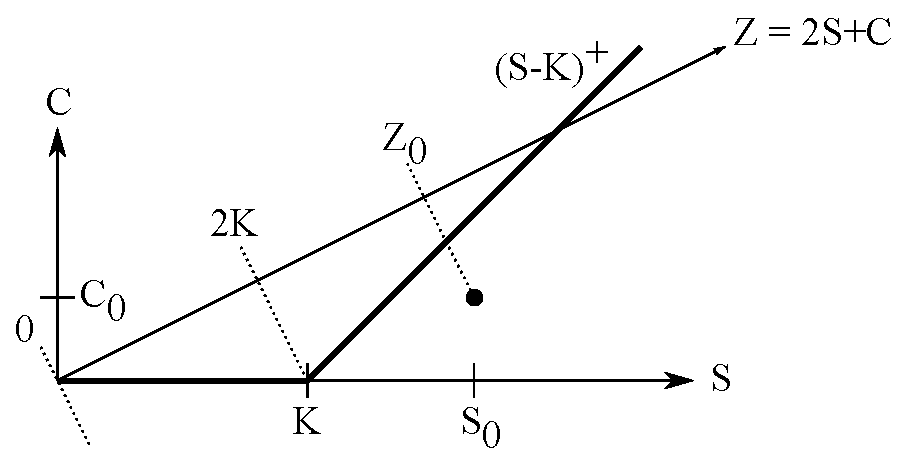
\includegraphics[width=3in]{Images/SC_21.eps}
  \caption[Stock-Call Space with (2,1) Portfolio]
          {Stock-Call Space with (2,1) Portfolio}
  \label{fig:SC_21}
\end{figure}

Orthogonal projection implies the existence of a null space hyperplane. A natural construction is that of a portfolio whose initial value lies in this null space. The initial cost of such a portfolio is zero. Suppose that a call option with strike price $K$ costs $C_0$ with underlying stock of initial cost $S_0$ and that $S_0 / C_0 = 5$, for example. A zero-cost portfolio is $\pi = (-1,5)$, that is, sell one share of stock and buy $5$ call options. This situation is depicted in figure \ref{fig:SC_Zero}. The zero-cost portfolio is represented by $Z = -S + 5C$. Notice that $min(Z) = -K$ and that if the final stock price $S_T$ is $2K$ instead of $K$ the value of the portfolio $Z$ jumps from $-K$ to $3K$, four multiples of $K$ since the portfolio contains $5$ calls and one shorted share of stock whereas the terminal stock price rising form $0$ to $K$ results in $Z$ falling from $0$ to $-K$ since it contains the shorted stock and $5$ out-of-the-money call options. 

The probability distribution of the example $Z$ is approximated in figure \ref{fig:SC_Zero_RV} where the negative-put-like behavior is shaded and marked with its total probability $q$ assuming $S_T$ is represented by a $LogNormal$ random variable. Notice in particular that the probability distribution of $Z$ is not recognizable as either $LogNormal$ nor truncated $LogNormal$.

\begin{figure}
  \centering
  \includegraphics[width=3in]{Images/SC_Zero.eps}
  \caption[Stock-Call Space with Zero-Cost Portfolio]
          {Stock-Call Space with Zero-Cost Portfolio}
  \label{fig:SC_Zero}
\end{figure}

\begin{figure}
  \centering
  \includegraphics[width=3in]{Images/SC_Zero_RV.eps}
  \caption[Probability Distribution of Zero-Cost Portfolio]
          {Probability Distribution of Zero-Cost Portfolio}
  \label{fig:SC_Zero_RV}
\end{figure}

\subsection{Black Scholes Construction: SPY Example}

The work on Levy-Stable distributions by Nolan \cite{nolan13} takes the daily prices of a particular stock (ticker: SPY) shown in figure \ref{fig:SPY}. The daily returns for SPY are plotted in figure \ref{fig:SPY_returns}.

\begin{figure}
  \centering
  \includegraphics[width=3in]{Images/SPY.eps}
  \caption[Stock Price (ticker symbol: SPY)]
          {Stock Price (ticker symbol: SPY)}
  \label{fig:SPY}
\end{figure}

According to Nolan \cite{nolan13} a good fit of the SPY returns is achieved by a mixture of a LogNormal distribution and a Levy-Stable distribution. Using the numeric random variable facilities of RICO to plot $LogNormal(0,\sigma) \times LevyStable(\alpha, \beta, \delta, \gamma)$ for the specific fit parameters cited by Nolan \cite{nolan13},
\begin{lstlisting}
alpha = 1.86034
beta  = -0.0919429
gamma = 0.00600552
sigma = 0.532775
delta = 0.000232571
u     = log(gamma)
LN    = LogNormalNumeric(0, sigma, 100)
LS    = LevyStableNumeric(alpha, beta, delta, gamma, 100)
LNS   = LN * LS
Plot().xrange(-.1, .15).plot(LNS).show()
\end{lstlisting}

\begin{figure}
  \centering
  \includegraphics[width=3in]{Images/SPY_returns.eps}
  \caption[Stock Price (ticker symbol: SPY) daily return distribution]
          {Stock Price (ticker symbol: SPY) daily return distribution}
  \label{fig:SPY_returns}
\end{figure}

\begin{figure}
  \centering
  \includegraphics[width=3in]{Images/SPY_returns_fit.eps}
  \caption[Stock Price (ticker symbol: SPY) daily return distribution]
          {Stock Price (ticker symbol: SPY) daily return distribution}
  \label{fig:SPY_returns_fit}
\end{figure}

\begin{figure}
  \centering
  \includegraphics[width=3in]{Images/SPY_purchase.eps}
  \caption[SPY one day in future given \$80/share price today]
          {SPY one day in future given \$80/share price today}
  \label{fig:SPY_purchase}
\end{figure}

The fit found by Nolan \cite{nolan13} is overlayed on the SPY returns histogram in figure \ref{fig:SPY_returns_fit}. Suppose the current price of SPY is \$80/share. Following the Black Scholes construction, the share price of SPY at $T = $ one day in the future is denoted $S_T$ defined as,
\begin{align*}
S_T = 80 \times LNS
\end{align*}
where $LNS$ is the LogNormal-LevyStable distribution given the fit data found by Nolan \cite{nolan13}. Continuing from the previous code listing, the dsitribution of $S_T$ is computed by RICO as in the following listing with the result is shown in figure \ref{fig:SPY_purchase}.
\begin{lstlisting}
ST = 80*exp(LNS)
Plot().xrange(77,84).yrange(0,.8).plot(ST).show()
\end{lstlisting}

\begin{figure}
  \centering
  \includegraphics[width=3in]{Images/SPY_purchase_split.eps}
  \caption[SPY one day in future given \$80/share price today]
          {SPY one day in future given \$80/share price today}
  \label{fig:SPY_purchase_split}
\end{figure}

Supposing that the strike price for a 1 day option on SPY is $K = \$79.50$. The probability distribution of $S_T$ is then split at $K$ into two pieces as shown in figure \ref{fig:SPY_purchase_split}. Let
\begin{align*}
q := P(S_T < K)
\end{align*}
In this case $q \approx 0.22$ and is represented by the shaded region of figure \ref{fig:SPY_purchase_split}. The payoff random variable of a 1-day European-style call option according to the Black-Scholes construction $C_T$ is the following function of $S_T$
\begin{align*}
C_T = [S_T - K]^+
\end{align*}
shown in figure \ref{fig:SPY_purchase_call}. Notice that $C_T$ is both discrete and continuously distributed. In particular,
\begin{align*}
P(C_T = 0) = q && P(C_T > 0) = 1-q
\end{align*}

\begin{figure}
  \centering
  \includegraphics[width=3in]{Images/SPY_purchase_call.eps}
  \caption[Call option payoff on one-day SPY]
          {Call option payoff on one-day SPY}
  \label{fig:SPY_purchase_call}
\end{figure}

The salient point of this example is that the next step of the Black-Scholes construction cannot be completed for ths example. The reason is that the expected value of the continuous portion of $C_T$ is infinite! For the fit parameters used in this example the LNS distribution is \emph{fat tailed} and our example ends without a price for the one-day call option, $C_T$.

In practice return rates do not necessarily follow a Gaussian distribution. The Black Scholes construction remains computable so long as expected values of truncated distributions are finite. Note in particular that Monte Carlo techniques may not expose this fact.


%%%%%%%%%%%%%%%%%%%%%%%%%%%%%%%%%%%%%%%%%%%%%%%%%%%%%%%%%%%%%%%%%%%%%%%%%%%%%%%%%%%%%%%%%%

\appendix
\chapter{Tables and Chairs, Sharply}
\section{An Exemplary 2D Sharp Example}

The example presented here is small enough to describe in full detail and incorporate many of the key features of algebraically correlated random variables described in this work. Presented in two stages, first with sharp inputs replicating an example from Gass \cite{gass75} and the second with algebraically correlated random variable inputs. We will then describe how the example may be generalized.

The basis for the tables and chairs example can be found in Gass \cite{gass75} wherein a decision must be made by a small furniture manufacturer under resource constraints. The choice is whether to manufacture tables or chair or some combination of both. The goal is to maximize the revenue from the sale of the tables and chairs assuming that all will be sold. The specifics are,

\begin{enumerate}
\item There is 400 board-feet of wood available.
\item There is 450 man-hours of labor available.
\item It takes 5 board-feet of wood and 10 man-hours of labor to make a chair.
\item It takes 20 board-feet of wood and 15 man-hours of labor to make a table.
\item Chairs sell for \$45 each.
\item Tables sell for \$80 each.
\end{enumerate}

Stating the problem in standard form according to Boyd \cite{boyd04}
and Greenberg \cite{greenberg95},

\begin{align*}
\text{maximize} && 45 x_c + 80 x_t\\
\text{s.t.}     && 5 x_c + 20 x_t \le 400\\
                && 10 x_c + 15 x_t \le 450\\
                && x_c, x_t \ge 0
\end{align*}

where $x_c$ represents the number of chairs to manufacture and sell
and $x_t$ represents the number of tables to manufacture and sell.

To form a baseline we will first solve this optimization problem using
the simplex method as described in the simplex method section. We will
then solve the problem again with the prices kept unknown. At that
point we will be ready to introduce random pricing into the problem.

\subsection{Tables and Chairs with All Inputs Sharp and Known}

The simplex method requires all constraints to be stated as equalities
so we introduce a slack variable into each inequality. The problem is
restated as,

\begin{align*}
\text{maximize} && 45 x_c + 80 x_t\\
\text{s.t.}     && 5 x_c + 20 x_t + s_W = 400\\
                && 10 x_c + 15 x_t + s_L\le 450\\
                && x_c, x_t, s_W, s_L \ge 0
\end{align*}

where $s_W$ is the slack variable for the wood resource equation and
$s_L$ is the slack variable for the labor resource equation. All
variables, $x_c$, $x_t$, $s_W$ and $s_L$ are constrained to be
non-negative.

Since each slack variable appears exclusively once in the constraint
equations and their coefficients are $+1$ they collectively form a
basis for the simplex tableau in table \ref{tab:tc0011}

\begin{table}
\centering
\begin{tabular}{| l | c c c c | c |}
\hline
        & $x_c$ & $x_t$ & $s_W$ & $s_L$ & $b$\\
\hline
$s_W$   & 5     & 20    & 1     & 0     & 400\\
$s_L$   & 10    & 15    & 0     & 1     & 450\\
\hline
Revenue & 45    & 80    & 0     & 0     &\\
\hline
\end{tabular}
  \caption[Tables and Chairs Simplex Tableau for State 0011]
          {Tables and Chairs Simplex Tableau for State 0011}
  \label{tab:tc0011}
\end{table}


The problem variables are collected into the list $X = (x_c, x_t, s_W,
s_L)$ and using the order of this list denote the variables in the
current basis with a $1$ and the others with a $0$ we describe the
current simplex state with the binary value,

\begin{align*}
State_0 = 0011
\end{align*}

To pivot the table we find the variable to enter the basis and the
basis variable to exit the basis. To find the entering variable we
compute the cost impact of each,

\begin{align*}
Z_c &= 45 - (5*0 + 10*0) &= 45\\
Z_t &= 80 - (20*0 + 15*0) &= 80
\end{align*}

where $Z_c$ is the cost impact of introducing variable $x_c$ into the
basis and $Z_t$ is the cost impact for $x_t$. Recall that increasing
$x_c$ the assumed zero value for a non-basis variable by one unit (one
more chair sold, for example) will increase revenue by the price of
one chair, $\$45$, and will decrease the slack variables $s_W$ and
$s_L$ by $5$ and $10$ units respectively. Since there is no revenue
impact to increasing or decreasing slack variables the revenue impact
is zero for each. 

The entering variable is selected as,
\begin{align*}
\text{argmax}\{Z_c, Z_t\} \implies x_t
\end{align*}

We now know that the next simplex state has the form $10??$ because
$x_c$ is the entering variable and where the question marks indicate
that we do no yet know the exiting variable. 

Since $x_t$ is the entering variable we divide $b = (400, 450)$
element-wise by the basis coefficients for $x_t$ namely $20$ and $15$
and find the minimum non-negative value. In particular one finds,
\begin{align*}
\text{argmin}\{\frac{400}{20}, \frac{450}{15}\} \implies s_W
\end{align*}

Since $\frac{400}{20} < \frac{450}{15}$ and the former value is
associated with basis variable $s_W$ it is chosen as the exit
variable. Recall that the reason is because we are allowing the
entering variable $x_t$ to increase from zero it forces the basis
variable in each equation toward zero. In the first equation a unit
increase in $x_t$ is a $20$ unit decrease in $s_W = 400$, but only a
$15$ unit decrease in $s_L = 450$. Since no variable is allowed to be
negative the we find which basis variable is driven to zero
first by an increase in the entering variable. We now see the new
simplex state to be,
\begin{align*}
State_1 = 0101
\end{align*}

To transform the equations and update the tableau we form the
transformation matrix to state $1$,  $B_1$ and its inverse as,
\begin{align*}
B_1 = \begin{pmatrix}20&0\\15&1\end{pmatrix} && B_1^{-1} = \frac{1}{20}\begin{pmatrix}1&0\\-15&20\end{pmatrix}
\end{align*}

recognizing each tableau column as a vector and multiplying on the
left by $B_1^{-1}$ we find the new tableau in table \ref{tab:tc0101}.

\begin{table}
\centering
\begin{tabular}{| l | c c c c | c |}
\hline
        & $x_c$ & $x_t$ & $s_W$ & $s_L$ & $b$\\
\hline
$x_t$   & $\frac{1}{4}$     & 1    & $\frac{1}{20}$     & 0     & 20\\
$s_L$   & 6$\frac{1}{4}$    & 0    & -$\frac{3}{4}$     & 1     & 150\\
\hline
Revenue & 45    & 80    & 0     & 0     &\\
\hline
\end{tabular}
  \caption[Tables and Chairs Simplex Tableau for State 0101]
          {Tables and Chairs Simplex Tableau for State 0101}
  \label{tab:tc0101}
\end{table}


The two non-basis variables are now $x_c$ and $s_W$ so we find the
cost impact for introducing each into the basis,

\begin{align*}
Z_c &= 45 - (\frac{1}{4}*80 + 6\frac{1}{4}*0) &= 25\\
Z_w &= 0 - (\frac{1}{20}*80 - \frac{3}{4}*0) &= -4 
\end{align*}

where $Z_w$ is the cost impact of (re)-introducing $s_W$ into the
basis. Since $Z_w$ is negative, $s_W$ it is not eligible to be a
basis vector leaving $x_c$ as the only available choice for entering
variable.

Dividing $b$ by the vector of coefficients associated with $x_c$ and
finding the smallest non-negative value we have,

\begin{align*}
\text{argmin}\{20 \div \frac{1}{4}, 150 \div 6\frac{1}{4}\} =
\text{argmin}\{80, 24\} \implies s_L
\end{align*}

demonstrating the $s_L$ is the exiting variable. The $B_2$ basis
transformation matrix and its inverse become,

\begin{align*}
B_2 = \begin{pmatrix}\frac{1}{4}&1\\6\frac{1}{4}&0\end{pmatrix} && B_2^{-1} = \begin{pmatrix}0&0.16\\1&-0.04\end{pmatrix}
\end{align*}

The simplex state is then,
\begin{align*}
State_2 = 1100
\end{align*}

and the tableau for state 1100 is shown in table \ref{tab:tc1100}.

\begin{table}
\centering
\begin{tabular}{| l | c c c c | c |}
\hline
        & $x_c$ & $x_t$ & $s_W$ & $s_L$ & $b$\\
\hline
$x_c$   & 1    & 0    & -0.12   & 0.16     & 24\\
$x_t$   & 0    & 1    & 0.08    & -0.04    & 14\\
\hline
Revenue & 45    & 80    & 0     & 0     &\\
\hline
\end{tabular}
  \caption[Tables and Chairs Simplex Tableau for State 1100]
          {Tables and Chairs Simplex Tableau for State 1100}
  \label{tab:tc1100}
\end{table}

We see that the two slack variables are no longer in the basis so they
are both zero. This means that at the current state we are using all
available resources to manufacture our tables and chairs. We ask if
either of the two slack variables should be re-introduced into the
basis by calculating the revenue impact for each,

\begin{align*}
Z_W &= 0 - (-0.12*45 + 0.08*80) &= -1\\
Z_L &= 0 - (0.16*45 - 0.04*80) &= -4
\end{align*}

Since each  cost impact is negative we conclude there is no possible
way to improve the revenue of the problem and the algorithm terminates
with the results,

\begin{align*}
x_c &= 24\\
x_t &= 14\\
revenue &= 24*45 + 14*80 = \$2,200
\end{align*}

since $(x_c, x_t) = b$. This means that the optimal choice for the
manufacturer is to make 24 chairs and 14 tables which, when sold, will
generate a revenue of $\$2,200$.

\begin{figure}
  \centering
  \includegraphics[width=120mm]{Images/tables_and_chairs}
  \caption[Tables and Chairs Constraints and Optimal Point]
          {Tables and Chairs Constraints and Optimal Point}
  \label{fig:tables_and_chairs}
\end{figure}

Figure \ref{fig:tables_and_chairs} shows the resource constraints
(diagonal lines), the feasible region (shaded area) and the optimal
point, $(24,14)$. The simplex method starts at the origin in this case
and follows the heavy line in figure \ref{fig:tables_and_chairs} from
vertex to vertex of the polytope described by the half-space
constraints to the optimal vertex. We notice that in this case there
is an alternate vertex-path from the origin to the optimal vertex,
namely passing through point $(45,0)$. We will see that the choice of
vertex-path is significant in the next version of this example when we
leave the prices unknown.

\subsection{Tables and Chairs with Unknown Prices}

As an intermediate step we consider where uncertainty may be injected
into the tables and chairs example and decide that leaving the prices
sharp, but unknown leads to some revealing results.

A priori there are three places in the tables and chairs example where
uncertainty may be injected; the constraint vector $b$, the price
vector $p$ and the constraint matrix $A$ where,

\begin{align*}
A &= \begin{pmatrix}5&20\\10&15\end{pmatrix}\\
b &= \begin{pmatrix}400\\450\end{pmatrix}\\
p &= \begin{pmatrix}45&80\end{pmatrix}
\end{align*}

We recognize the values in the $A$ matrix as the amount of resources
of each type consumed to manufacture each kind of product, $b$ is the
number of resources of each kind available and $p$ is the prices
charged for each product.

Suppose that instead of the $5$ in matrix $A$ we introduced a random
variable. In the context of the tables and chairs example this means
that the manufacturer is uncertain about the amount of wood necessary
to construct a chair. We assume there is only one kind of chair else we
would likely call out the different kinds as different products and
give them separate variables. We make similar statements about each
value in the $A$ matrix. 

Since we are most interested in reflecting the AB32 reference model
into the tables and chairs example we elect not to introduce random
variables into the $A$ matrix. The reason is that the corresponding
$A$ matrix of the AB32 model represents policy features and physical
limitations which are assumed for the given policy under
consideration. 

To choose to introduce random variables into the $b$ or $p$ vectors we
must understand how they are used within the simplex algorithm. The
simplex method uses a \emph{pivot-table} approach whereby a column and
related row within the simplex tableau are chosen and a transition is
made to a new state within the algorithm. 

To choose the simplex tableau column we compare revenue impacts given
a choice of one of the non-basis variables. The values involved in
computing the revenue impact of each non-basis variable are prices and
products of prices and $A$ matrix coefficients from columns
corresponding to the non-basis variables. If we assume that the $A$
matrix values are fixed then we are comparing linear combinations of
$p$ vector prices to find the  non-basis variable corresponding to the
non-negative maximum of revenue impact values.

To choose the simplex tableau row given a column choice we compute the
quotient of $b$ and the values in $A$ corresponding to that
column. Thus we are comparing linear combinations of $b$ vector
values to find the basis variable corresponding to the the non-negative
minimum of linear combinations of constraint values.

We thus see that $p$ and $b$ values do not interact directly within
the simplex method. We will then choose the $p$ vector for
introduction of random variables suggesting, in the tables and chairs
example, price uncertainty over the $b$ vector values which would
suggest resource uncertainty. We will see that no new insight is
gained though choosing $b$ over $p$ or through choosing both for
random variable introduction. We will comment below on the choice of
$A$ for random variable introduction especially if $p$ or $b$ are
chosen as well. 

For this intermediate tables and chairs example we have unknown, but
sharp prices $p_c$ and $p_t$ for chairs and tables respectively. We
make one assumption about these unknown prices; they are positive. The
problem may then be stated in standard form as,

\begin{align*}
\text{maximize} && p_c * x_c + p_t * x_t\\
\text{s.t.}     && 5 x_c + 20 x_t \le 450\\
                && 10 x_c + 15 x_t \le 450\\
                && x_c, x_t \ge 0\\
                && p_c, p_t > 0
\end{align*}

The initial simplex tableau is shown in table \ref{tab:tcp0011}. The
only differences from the initial tableau of the first example is the
introduction of the state value $0011$ into the upper-left corner and
the unknown prices $p_c$ and $p_t$.

\begin{table}
\centering
\begin{tabular}{| l | c c c c | c |}
\hline
0011    & $x_c$ & $x_t$ & $s_W$ & $s_L$ & $b$\\
\hline
$s_W$   & 5     & 20    & 1     & 0     & 400\\
$s_L$   & 10    & 15    & 0     & 1     & 450\\
\hline
Revenue & $p_c$ & $p_t$ & 0     & 0     &\\
\hline
\end{tabular}
  \caption[Tables and Chairs Simplex Tableau for State 0011 with Unknown Prices]
          {Tables and Chairs Simplex Tableau for State 0011 with Unknown Prices}
  \label{tab:tcp0011}
\end{table}

Following the steps from the first example we must find the entering
non-basis variable by finding,

\begin{align*}
  &\text{argmax}\{p_c - (5*0 + 10*0), p_t - (20*0 + 15*0)\}\\
= &\text{argmax}\{p_c, p_t\}
\end{align*}

Since $p_c, p_t > 0$ neither case may be disqualified so we have some
possibilities. Either $p_c < p_t$ or $p_c > p_t$ or $p_c = p_t$. Since
we intend, in the next example, to introduce continuous random
variables in place of $p_c$ and $p_t$, equality occurs with
probability zero so we ignore that case here.

If $p_c > p_t$ then we choose $x_c$ as the entering variable. To find
the exiting variable we compute,

\begin{align*}
  &\text{argmin}\{\frac{400}{5}, \frac{450}{10}\}\\
= &\text{argmin}\{80, 45\} \implies s_L
\end{align*}

Since we have chosen $x_c$ as the entering variable and $s_L$ as the
exiting variable our new state is $1010$ and the transition matrix $B_{1010}$
and its inverse $B_{1010}^{-1}$ is,

\begin{align*}
B_{1010} = \begin{pmatrix}5&1\\10&0\end{pmatrix} && B_{1010}^{-1} = \frac{1}{10}\begin{pmatrix}0&1\\10&-5\end{pmatrix}\end{align*}

The new $1010$ tableau is shown in table \ref{tab:tcp1010}.

\begin{table}
\centering
\begin{tabular}{| l | c c c c | c |}
\hline
1010    & $x_c$ & $x_t$ & $s_W$ & $s_L$ & $b$\\
\hline
$x_c$   & 1     & 1.5    & 0     & 0.1   & 45\\
$s_W$   & 0     & 12.5   & 1     & -0.5  & 175\\
\hline
Revenue & $p_c$ & $p_t$ & 0     & 0     &\\
\hline
\end{tabular}
  \caption[Tables and Chairs Simplex Tableau for State 1010 with Unknown Prices]
          {Tables and Chairs Simplex Tableau for State 1010 with Unknown Prices}
  \label{tab:tcp1010}
\end{table}

The non-basis variables are $x_t$ and $s_L$ so we compute the revenue
of (re)-introducing each of them, respectively, and find the entering variable,

\begin{align*}
   \text{argmax}\{p_t - (1.5*p_c + 12.5*0), 0 - (0.1*p_c - 0.5*0)\}
= &\text{argmax}\{p_t - 1.5*p_c , - 0.1*p_c\}
\end{align*}

Since $p_c > 0$ by assumption we have $-0.1*p_c < 0$ so it must be
disqualified as an option. We then ask, under what condition is the
first options positive? That is,

\begin{align*}
p_t - 1.5*p_c &> 0\\
p_t &> 1.5*p_c\\
\frac{2}{3}p_t &> p_c
\end{align*}

Since we have already assumed upon entering this case that $p_c > p_t$
it is not possible for $\frac{2}{3}p_t > p_c$. We therefore terminate
the simplex algorithm. Recalling that non-basis variables must be zero
we find the following results,

\begin{align*}
x_c &= 45\\
x_t &= 0\\
revenue &= 45p_c && \text{ for } p_t < p_c
\end{align*}

Returning to our first decision point we now assume $p_c < p_t$ as was
the case in the first example. The tableau under the assumption that
we transition from state $0011$ to state $0101$ is shown in table
\ref{tab:tcp0101} which we notice is similar to table
\ref{tab:tc0101} except for the unknown prices and the state being
recorded in the upper left corner of the tableau.

\begin{table}
\centering
\begin{tabular}{| l | c c c c | c |}
\hline
0101    & $x_c$ & $x_t$ & $s_W$ & $s_L$ & $b$\\
\hline
$x_t$   & $\frac{1}{4}$     & 1    & $\frac{1}{20}$     & 0     & 20\\
$s_L$   & 6$\frac{1}{4}$    & 0    & -$\frac{3}{4}$     & 1     & 150\\
\hline
Revenue & $p_c$   & $p_t$    & 0     & 0     &\\
\hline
\end{tabular}
  \caption[Tables and Chairs Simplex Tableau for State 0101 with Unknown Prices]
          {Tables and Chairs Simplex Tableau for State 0101 with Unknown Prices}
  \label{tab:tcp0101}
\end{table}

From state $0101$ the non-basis variables are $x_c$ and $s_W$ so we
compute the revenue maximizing variables by the usual methods,

\begin{align*}
&\text{argmax}\{p_c - (\frac{1}{4}p_t + 6\frac{1}{4}*0), 0 -
(\frac{1}{20}p_t - \frac{3}{4}*0)\}\\
= &\text{argmax}\{p_c - \frac{1}{4}p_t, -\frac{1}{20}p_t\}
\end{align*}

Since $p_t > 0$ the second option of $-\frac{1}{20}*p_t < 0$ and is
disqualified. From the first option we conclude that if $p_c <
\frac{1}{4}*p_t$ that the simplex algorithm terminates. The results of
this termination are,

\begin{align*}
x_c &= 0\\
x_t &= 20\\
revenue &= 20p_t && \text{ for } p_c < \frac{1}{4}p_t
\end{align*}

For the simplex algorithm to not terminate at this part requires that
$p_c > \frac{1}{4}p_t$. Recall that we are already operating under the assumption
that $p_c < p_t$. Since these two assumptions are compatible (i.e. not
impossible) we continue the simplex algorithm. From the calculation
for entering variable we conclude that $x_c$ is the entering variable
and we must find the exiting variable. Since we have seen this exact
situation in the first example we simply recall the result that $s_L$
is the exiting variable and that the resulting tableau is shown in
table \ref{tab:tcp1100}. Because we are in the same state as before this
new figure is nearly identical to the previous table \ref{tab:tc1100}.

\begin{table}
\centering
\begin{tabular}{| l | c c c c | c |}
\hline
1100    & $x_c$ & $x_t$ & $s_W$ & $s_L$ & $b$\\
\hline
$x_c$   & 1    & 0    & -0.12   & 0.16     & 24\\
$x_t$   & 0    & 1    & 0.08    & -0.04    & 14\\
\hline
Revenue & $p_c$ & $p_t$    & 0     & 0     &\\
\hline
\end{tabular}
  \caption[Tables and Chairs Simplex Tableau for State 1100 with Unknown Prices]
          {Tables and Chairs Simplex Tableau for State 1100 with Unknown Prices}
  \label{tab:tcp1100}
\end{table}

In the first example, once we reached this state (1100) the simplex
algorithm terminated. As before we attempt to find the entering
variable with the calculation,

\begin{align*}
&\text{argmax}\{0 - (-0.12p_c + 0.08p_t), 0 - (0.16p_c - 0.04p_t)\}\\
= &\text{argmax}\{0.12p_c - 0.08p_t, 0.04p_t - 0.16p_c\}\\
= &\text{argmax}\{3p_c - 2p_t, p_t - 4p_c\}
\end{align*}

For the second option to be positive and therefore available for
consideration requires that $p_t > 4p_c$ which is to say $p_c <
\frac{1}{4}p_t$. However, to reach this state we assumed $p_c >
\frac{1}{4}p_t$ so the second option is not available.

If $p_c < \frac{2}{3}p_t$ then the simplex algorithm terminates just
as it did in the first example since $45 < \frac{2}{3}*80 =
53.33...$. The result in this case is,

\begin{align*}
x_c &= 14\\
x_t &= 24\\
revenue &= 14p_c + 24p_t && \text{ for } \frac{1}{4}p_t < p_c < \frac{2}{3}p_t
\end{align*}

If $\frac{2}{3}p_t < p_c$ then the first option for the entering
variable is available and the entering variable is found to be $s_W$.

The exiting variable in this case is then found as,

\begin{align*}
\text{argmin}\{24 \div -0.12, 14 \div 0.08\}
\end{align*}

Since the first option is negative it is disqualified leaving the
second option and therefore the second of the two basis variables
$x_t$ as the exiting variable. 

Pivoting on the $s_W$ column and the $x_t$ row we have the transition
matrix $B_{1010}$ and its inverse $B_{1010}^{-1}$ as,

\begin{align*}
B_{1010} = \begin{pmatrix}1&-0.12\\0&0.08\end{pmatrix} && 
B_{1010}^{-1} = \begin{pmatrix}1&1.5\\0&125.5\end{pmatrix}
\end{align*}

Applying our transition matrix $B_{1010}^{-1}$ to the $1100$ state
tableau return us to the $1010$ state tableau shown in figure
\ref{tab:tcp1010}.  Since we have determined that state $1010$
terminates we have the following results,

\begin{align*}
x_c &= 45\\
x_t &= 0\\
revenue &= 45p_c && \text{ for } \frac{2}{3}p_t < p_c < p_t
\end{align*}

Because we followed a different path between states to arrive at state
$1010$, the conditions for reaching this state are different. We
notice that the conditions for reaching this state directly from the
initial $0011$ state are $p_t < p_c$ do not intersect the conditions
for reaching this state from state $1010$ as we have just
completed. We combine the two conditions to see that the revenue
outcome of $45p_c$ is reached if $\frac{2}{3}p_t < p_c$.

The result of our investigation is that there are three possible cases
for any pair of positive prices given that all other values in the
tables and chairs example remain the same, that is,

\begin{align*}
\text{Revenue } = \begin{cases}45p_c & \text{ if } \frac{2}{3}p_t < p_c\\
  24p_c + 14p_t & \text{ if } \frac{1}{4}p_t < p_c < \frac{2}{3}p_t\\
  20p_t & \text{ if } p_c < \frac{1}{4}p_t\end{cases}
\end{align*}

The results of this example are summarized by the directed graph in figure
\ref{fig:tc_directed_graph}. The nodes of the graph are the states of
the simplex algorithm allied to this example, the edges are marked
with the conditions under which the simplex algorithm will follow the
edge and the three output cases are labeled $A$, $B$ and $C$
accompanied by the resulting revenue.

\begin{figure}
  \centering
  \includegraphics[width=3in]{Images/tc_directed_graph}
  \caption[Tables and Chairs Directed Graph]
          {Tables and Chairs Directed Graph}
  \label{fig:tc_directed_graph}
\end{figure}

Looking ahead, suppose we were given random variables $P_t$ and $P_c$
representing the price of tables and chairs respectively. Even if
$P_t$ and $P_c$ are correlated in some manner they have a joint
distribution which we represent as the shaded region in figure
\ref{fig:tc_joint_prices}. The figure (\ref{fig:tc_joint_prices}) has
three levels of shading with each region labeled with its outcome
($A$, $B$ or $C$) corresponding to the directed graph in figure
\ref{fig:tc_directed_graph}. We note that if the two price random
variables are independent then the shaded region representing the
joint probability distribution of $P_t$ and $P_c$ would be
rectangular. 

\begin{figure}
  \centering
  \includegraphics[width=3in]{Images/tc_joint_prices}
  \caption[Tables and Chairs Partitioned Price Probability Space]
          {Tables and Chairs Partitioned Price Probability Space}
  \label{fig:tc_joint_prices}
\end{figure}



%%%%%%%%%%%%%%%%%%%%%%%%%%%%%%%%%%%%%%%%%%%%%%%%%%%%%%%%%%%%%%%%%%%%%%%%%%%%%%%%%%%%%%%%%%
\bibliographystyle{plain}
\bibliography{Memoir}
%%%%%%%%%%%%%%%%%%%%%%%%%%%%%%%%%%%%%%%%%%%%%%%%%%%%%%%%%%%%%%%%%%%%%%%%%%%%%%%%%%%%%%%%%%
\end {document}
